%%%%%%%%%%%%%%%%%%%%%%%%%%%%%%%%%%%%%%%%%%%%%%%%%%%%%%%%%%%%%%%%%%%%%%%%%
\documentclass[12pt,a4paper,final]{extreport}
\usepackage[utf8]{inputenc}
\usepackage{amsmath}
\usepackage{amsfonts}
\usepackage{amssymb}
\usepackage{bm}
\usepackage{array}
\usepackage{setspace}
\usepackage{verbatim}
\usepackage{adjustbox}
\usepackage{multirow}
\usepackage{caption}
\usepackage{subcaption}
\usepackage{ragged2e}
\justifying
\usepackage{tabularx}
\usepackage{booktabs}
\usepackage{float}
\usepackage{longtable}
\usepackage[table]{xcolor}
\renewcommand{\bibname}{References}
\usepackage[colorlinks]{hyperref}
\hypersetup{linkcolor={black},citecolor={black},urlcolor={black}}
\usepackage{graphicx}
\usepackage[left=3cm,right=2cm,top=3cm,bottom=3.5cm]{geometry}
\linespread{1.5}
\usepackage{titlesec}
\usepackage[yyyymmdd]{datetime}
\usepackage{fancyhdr}
\setlength{\headheight}{15pt}
\usepackage{algorithm}
\usepackage{algpseudocode}
\usepackage{enumitem}
\setlist{itemsep=2pt,topsep=4pt,parsep=0pt}
\usepackage{tikz}
\usetikzlibrary{arrows.meta,positioning,shapes.geometric,fit,calc,backgrounds}
\usepackage{pgfplots}
\pgfplotsset{compat=1.18}
\pgfplotsset{every axis/.append style={x tick label style={text height=1.6ex, text depth=0.35ex}}}

% --- Chart colours (validated categorical slots 1 and 2) ---
\definecolor{seriesA}{HTML}{2A78D6}   % baselines / series 1
\definecolor{seriesB}{HTML}{EB6834}   % proposed method / series 2
\definecolor{gridgray}{HTML}{D9D9D6}
\definecolor{seriesC}{HTML}{1BAF7A}   % series 3
\definecolor{seriesD}{HTML}{EDA100}   % series 4
\definecolor{inkgray}{HTML}{52514E}
% --- Diagram fills ---
\definecolor{boxblue}{HTML}{E3EEFB}
\definecolor{boxorange}{HTML}{FCE8DE}
\definecolor{boxgreen}{HTML}{DFF3EA}
\definecolor{boxgray}{HTML}{F1F1EF}
\definecolor{boxviolet}{HTML}{E9E6F7}

% --- Float placement: let text fill pages instead of leaving gaps ---
\renewcommand{\topfraction}{0.85}
\renewcommand{\bottomfraction}{0.7}
\renewcommand{\textfraction}{0.1}
\renewcommand{\floatpagefraction}{0.75}
\setcounter{topnumber}{3}
\setcounter{bottomnumber}{2}
\setcounter{totalnumber}{4}
\setlength{\textfloatsep}{14pt plus 4pt minus 4pt}
\setlength{\floatsep}{12pt plus 4pt minus 2pt}
\setlength{\intextsep}{12pt plus 4pt minus 2pt}
\captionsetup{font=small,labelfont=bf,skip=6pt}
\raggedbottom
\setlength{\emergencystretch}{2.5em}
\makeatletter
\renewcommand*\l@figure{\@dottedtocline{1}{1.5em}{3.3em}}
\makeatother

% --- Custom figure numbering format ---
\usepackage{chngcntr}          % allows linking counters
\counterwithin{figure}{section} % make figure numbering depend on section number
\renewcommand{\thefigure}{\thesection.\arabic{figure}} % custom figure numbering format

% Title/section formatting (matching sample)
\titleformat{\chapter}[display]
{\normalfont\rmfamily\huge\bfseries\color{black}}
{\chaptertitlename\ \thechapter}{20pt}{\huge}
\titleformat{\section}
{\normalfont\rmfamily\normalsize\bfseries\color{black}}
{\thesection}{16pt}{\large}
\titleformat{\subsection}
{\normalfont\rmfamily\small\bfseries\color{black}}
{\thesubsection}{16pt}{\normalsize}

\titlespacing{\chapter}{0pc}{0pc}{.5pc}
\titlespacing{\section}{0pc}{.8pc}{.2pc}
\titlespacing{\subsection}{0pc}{.8pc}{.1pc}

\thispagestyle{empty}
\begin{document}

% ================= TITLE PAGE =================
\begin{titlepage}
    \centering % Center all content on the page
    \pagenumbering{gobble} % Ensure no page number

    % --- Title and Subtitle ---
    {\Large\textbf{Multimodal AI with Computer Vision}} \\
    \vspace*{0.4 cm}
    {\large\textbf{SEMINAR REPORT}} \\
    \vspace*{0.7cm}

    % --- Author Block ---
    {\emph{Submitted by}}\\[0.2cm]
    \textbf{Ananda Padmanabhan PB}\\
    \textbf{SNM23CA008}\\
    \textbf{to}\\
    \textbf{the APJ Abdul Kalam Technological University}\\
    \textbf{in partial fulfillment of the requirements for the award of the Degree of}\\
    \textbf{Bachelor of Technology}\\
    \textbf{in}\\
    \textbf{Computer Science and Engineering (Artificial Intelligence)}\\
    \vspace*{0.7cm}

    % --- Guidance Block ---
    {\textit{Under the guidance of}} \\[0.15cm]
    \textbf{Ms. Surya T S} \\
    \textbf{Assistant Professor} \\
    \textbf{Dept. of CSE} \\
    \vspace*{0.6cm}

    % --- Image ---
    
\includegraphics[scale=0.42]{snm.jpg} \\
    \vspace*{.6cm}

    % --- Department and College ---
    \textbf{Department of Computer Science and Engineering (Artificial Intelligence)} \\
    \textbf{SREE NARAYANA MANGALAM INSTITUTE OF}\\
    \textbf{MANAGEMENT AND TECHNOLOGY}\\
    \textbf{MALIANKARA}\\
    \vspace*{0.8cm}

    % --- Date ---
    October 2026

    \vfill
\end{titlepage}

% ================= CERTIFICATE =================
\clearpage
\thispagestyle{empty}
\begin{center}
{\fontsize{13}{16}\selectfont \textbf{DEPARTMENT OF COMPUTER SCIENCE \& ENGINEERING\\(ARTIFICIAL INTELLIGENCE)}}\\[10pt]
{\fontsize{13}{16}\selectfont \textbf{SREE NARAYANA MANGALAM INSTITUTE OF MANAGEMENT \&\\TECHNOLOGY, MALIANKARA}}\\[14pt]

\includegraphics[scale=0.32]{snm.jpg}\\[10pt]
\textbf{\Large CERTIFICATE}
\end{center}
\vspace{4pt}

\begingroup\setstretch{1.35}
\noindent\emph{This is to certify that the seminar report entitled {\bf{Multimodal AI with Computer Vision}} submitted by {\bf Ananda Padmanabhan PB} ({\bf SNM23CA008}), to the {\bf Department of Computer Science and Engineering (Artificial Intelligence), SNM Institute of Management and Technology, Maliankara}, in partial fulfilment of the requirement for the award of B.Tech Degree in Computer Science and Engineering (Artificial Intelligence) is a bonafide record of the work carried out by the student.}\par
\endgroup

\vspace{1.8cm}

% Guide and HOD: each block is centred within its own half of the page
\noindent
\begin{minipage}[t]{0.48\textwidth}
\centering
\textbf{Guide}\\[28pt]
\textbf{Ms. Surya T S}\\
\textbf{Asst. Professor}\\
\textbf{Dept. of CSE}
\end{minipage}%
\hfill
\begin{minipage}[t]{0.48\textwidth}
\centering
\textbf{Head of the Department}\\[28pt]
\textbf{Ms. Lakshmi Anand}\\
\textbf{Asst. Professor}\\
\textbf{Dept. of CSE}
\end{minipage}

\vspace{1.1cm}

\noindent
\begin{minipage}[t]{\textwidth}
\centering
\textbf{Coordinator}\\[28pt]
\textbf{Ms. Surya T S}\\
\textbf{Asst. Professor}\\
\textbf{Dept. of CSE}
\end{minipage}

\newpage

% ================= DECLARATION =================
\thispagestyle{empty}
\begin{center}
\begin{huge}
\textbf{Declaration}
\end{huge}
\end{center}

\vskip0.5cm
I undersigned hereby declare that the seminar report \textbf{Multimodal AI with Computer Vision}, submitted for partial fulfilment of the requirements for the award of degree of Bachelor of Technology of the APJ Abdul Kalam Technological University, Kerala is a bonafide work done by me under the supervision of \textbf{Ms. Surya T S}. This submission represents my ideas in my own words and where ideas or words of others have been included, I have adequately and accurately cited and referenced the original sources. I also declare that I have adhered to ethics of academic honesty and integrity and have not misrepresented or fabricated any data or idea or fact or source in my submission. I understand that any violation of the above will be a cause for disciplinary action by the institute and/or the University and can also evoke penal action from the sources which have thus not been properly cited or from whom proper permission has not been obtained. This report has not been previously formed the basis for the award of any degree, diploma or similar title of any other University.

\vspace{2cm}
\noindent
\begin{minipage}[t]{0.5\textwidth}
Place: Maliankara\\
Date: 23/10/2026
\end{minipage}%
\hfill
\begin{minipage}[t]{0.4\textwidth}
\centering
\textbf{Ananda Padmanabhan PB}\\
\textbf{SNM23CA008}
\end{minipage}

\newpage
\thispagestyle{plain}
\pagenumbering{Roman}
\setcounter{page}{1}
\addcontentsline{toc}{chapter}{Acknowledgement}
\begin{center}
\begin{huge}
\textbf{Acknowledgement}
\end{huge}
\end{center}
\vskip1cm
\hspace*{1 cm} Firstly, I thank God, the Almighty, with whose blessings, this seminar has been successfully completed.

I wish to give deep sense of acknowledgement to our Principal \textbf{Dr. Atmaram P}, for his constant encouragement and valuable advice throughout the course.

I am extremely grateful to \textbf{Ms. Lakshmi Anand}, Head of the Department of Computer Science and Engineering, for the valuable guidance through this humble endeavor. The highly enterprising attitude, patience for listening to my doubts, timely suggestions and guidance made my seminar a so-called reality in stipulated time.
I would also like to thank our seminar coordinator and my seminar guide \textbf{Ms. Surya T S}, Assistant Professor, Department of Computer Science and Engineering, for the gracious encouragement and the valuable assistance.

I express my sincere gratitude to all the faculty members of the department of Computer Science and Engineering (Artificial Intelligence) for their co-operation and support to the seminar.

I also express my sincere gratitude to all my friends and my parents for their co-operation and constant inspiration.

\vspace{2cm}
\noindent\hfill
\begin{minipage}[t]{0.4\textwidth}
\centering
\textbf{Ananda Padmanabhan PB}
\end{minipage}

\newpage

% ================= ABSTRACT =================
\begin{center}
\begin{huge}
\textbf{Abstract}
\end{huge}
\end{center}

\addcontentsline{toc}{chapter}{Abstract}
\vskip0.3cm

\begingroup
\setstretch{1.15}
\paragraph{} Recent advancements in Multimodal Artificial Intelligence (AI) have significantly improved the ability of intelligent systems to understand, interpret, and reason using information from multiple modalities such as images, video, and text. This seminar presents a comprehensive review of four recent research works that collectively enhance multimodal AI through latent visual reasoning, perception-aware learning, efficient computation, and video-based pretraining.

\paragraph{} The Mirage framework introduces the concept of Machine Mental Imagery, enabling Vision-Language Models (VLMs) to perform multimodal reasoning using latent visual tokens instead of explicit image generation, thereby improving reasoning while avoiding the overhead of pixel-level synthesis. The AURORA framework enhances visual reasoning by introducing perception tokens that represent intermediate visual information such as depth maps and object locations, enabling more accurate spatial reasoning and object counting. ZipVL addresses the computational and memory challenges of large Vision-Language Models by dynamically selecting important visual tokens layer by layer, accelerating inference through adaptive token sparsity without significantly affecting accuracy. LLaVA-Prime shows that pretraining VLMs on large-scale video with causal hierarchical aggregation strengthens both temporal and static visual understanding.

\paragraph{} Together, these research contributions demonstrate how latent reasoning, perception-aware learning, efficient computation, and richer training data can be integrated to build more accurate, efficient, and reliable multimodal intelligent systems capable of addressing complex real-world applications across computer vision, robotics, healthcare, autonomous systems, and human-computer interaction.

\vspace{0.5cm}
\noindent
\textbf{Keywords:} Multimodal AI; Vision-Language Models; Multimodal Reasoning; Latent Visual Tokens; Perception Tokens; Dynamic Token Sparsity; Video Pretraining; Computer Vision; Deep Learning; Artificial Intelligence.
\endgroup

\newpage

% ================= TOC / LISTS =================
\thispagestyle{plain}
\begingroup
\setstretch{1.04}
\tableofcontents
\endgroup
\begingroup
\setstretch{1.2}
\listoffigures
\addcontentsline{toc}{chapter}{List of Figures}
\listoftables
\addcontentsline{toc}{chapter}{List of Tables}
\endgroup

% ================= LIST OF ABBREVIATIONS =================
\chapter*{List of Abbreviations}
\addcontentsline{toc}{chapter}{List of Abbreviations}

\begingroup
\setstretch{1.25}
\setlength{\LTleft}{0pt}\setlength{\LTright}{\fill}
\begin{longtable}{p{2.6cm}l}
\textbf{AI} & Artificial Intelligence \\
\textbf{CHA} & Causal Hierarchical Aggregation \\
\textbf{CLIP} & Contrastive Language-Image Pre-training \\
\textbf{CoT} & Chain-of-Thought \\
\textbf{CV} & Computer Vision \\
\textbf{FLOPs} & Floating-Point Operations \\
\textbf{GPU} & Graphics Processing Unit \\
\textbf{GRPO} & Group Relative Policy Optimisation \\
\textbf{InfoNCE} & Info Noise-Contrastive Estimation \\
\textbf{KV} & Key-Value (cache) \\
\textbf{LLM} & Large Language Model \\
\textbf{LVLM} & Large Vision-Language Model \\
\textbf{MLM} & Multimodal Language Model \\
\textbf{MLP} & Multi-Layer Perceptron \\
\textbf{RL} & Reinforcement Learning \\
\textbf{SFT} & Supervised Fine-Tuning \\
\textbf{t-SNE} & t-Distributed Stochastic Neighbour Embedding \\
\textbf{TTFT} & Time-to-First-Token \\
\textbf{ViT} & Vision Transformer \\
\textbf{VLM} & Vision-Language Model \\
\textbf{VQ-VAE} & Vector-Quantised Variational Autoencoder \\
\textbf{VQA} & Visual Question Answering \\
\textbf{VSP} & Visual-Spatial Planning \\
\end{longtable}
\endgroup

\newpage

% ================= PAGE STYLE =================
\lhead{Multimodal AI with Computer Vision}
\chead{}
\rhead{}
\lfoot{\textit{Dept. of CSE (AI), SNMIMT}}
\cfoot{}
\rfoot{\thepage}
\renewcommand{\headrulewidth}{0.4pt}
\renewcommand{\footrulewidth}{0.4pt}
\pagestyle{fancy}
\fancypagestyle{plain}{%
  \fancyhf{}%
  \lfoot{\textit{Dept. of CSE (AI), SNMIMT}}%
  \rfoot{\thepage}%
  \renewcommand{\headrulewidth}{0pt}%
  \renewcommand{\footrulewidth}{0.4pt}}
\titleformat{\chapter}[display]
  {\normalfont\huge\bfseries\filcenter}
  {\chaptername\ \thechapter}{1ex}{\Huge}
\titlespacing*{\chapter}{0pt}{-10pt}{24pt}

\pagenumbering{arabic}
\setcounter{page}{1}


% ================= CHAPTER 1: INTRODUCTION =================
\chapter{Introduction}

\paragraph{} For most of its history, computer vision built separate models for separate tasks: one network classified images, another detected objects, and a third estimated depth. \textbf{Multimodal Artificial Intelligence} (AI) changes this picture by learning from, and reasoning across, several kinds of data at once---images, video, and natural language. Its central building block is the \textbf{Vision-Language Model} (VLM), which encodes an image into a sequence of visual tokens and passes them, together with text, to a large language model (LLM) that can answer questions, describe scenes, and follow instructions \cite{liu2023,radford2021}.

\paragraph{} Today's VLMs are impressive generalists, but they reason almost entirely in \emph{words}, which suits description but not spatial planning \cite{p1}; they are weak at \emph{perception} such as judging depth or counting \cite{p2}; they are \emph{expensive}, because high-resolution images and videos produce thousands of visual tokens \cite{p3}; and their image-text training data teaches little about how scenes change over time \cite{p4}.

\paragraph{} This seminar reviews four recent works from CVPR and ICCV that address these limitations. Paper \cite{p1}, the base paper, by Yang et al., introduces \textbf{Mirage}, which lets a VLM ``think visually'' with latent visual tokens instead of generating images. Paper \cite{p2}, by Bigverdi et al., introduces \textbf{AURORA}, which teaches a VLM to produce \emph{perception tokens} such as depth maps and bounding boxes as intermediate reasoning steps. Paper \cite{p3}, by He et al., presents \textbf{ZipVL}, which accelerates VLM inference through dynamic token sparsity. Paper \cite{p4}, by Zhang et al., presents \textbf{LLaVA-Prime}, which scales VLM pretraining with video.

\section{General Background}

\paragraph{} Figure~\ref{fig:vlm} shows the typical VLM pipeline that all four works build on. A \textbf{vision encoder}, usually a Vision Transformer (ViT) \cite{dosovitskiy2021} pretrained with CLIP-style contrastive learning \cite{radford2021}, splits the image into patches and turns them into feature vectors. A small \textbf{projector}, often a multi-layer perceptron (MLP), maps these features into the LLM's embedding space, producing \textbf{visual tokens}. The LLM then processes visual and text tokens together and generates the answer one token at a time \cite{liu2023}. Each of the reviewed works intervenes at a different point in this pipeline: \cite{p4} at pretraining of the encoder and LLM, \cite{p3} at the attention computation inside the LLM, and \cite{p1,p2} at the output, by letting the model emit new kinds of tokens while it reasons.

\begin{figure}[htbp]
\centering
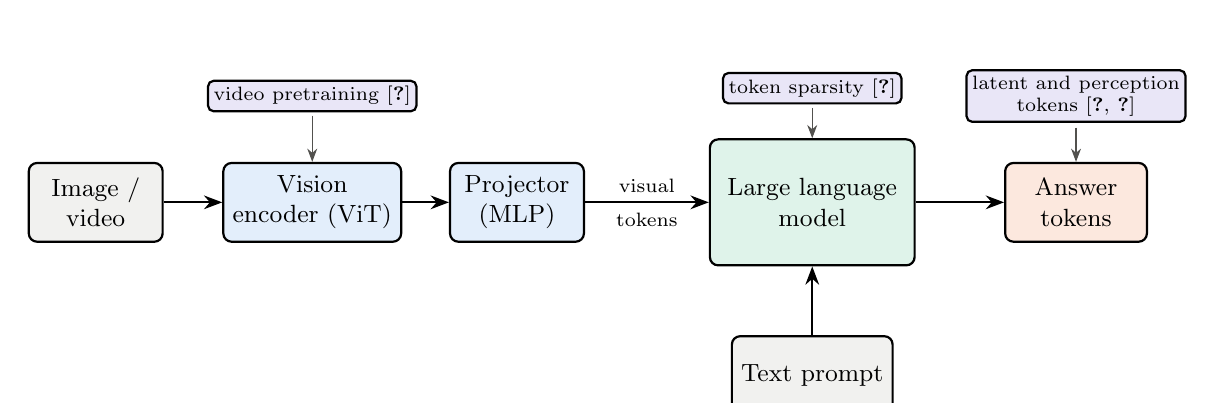
\begin{tikzpicture}[>=Stealth, thick,
  blk/.style={draw, rounded corners=3pt, minimum height=1.0cm, font=\small, align=center},
  tag/.style={draw, rounded corners=2pt, fill=boxviolet, font=\scriptsize, align=center, inner sep=2pt}]
\node[blk, fill=boxgray, minimum width=1.7cm] (img) at (0,0) {Image /\\ video};
\node[blk, fill=boxblue, minimum width=2.1cm] (enc) at (2.75,0) {Vision\\ encoder (ViT)};
\node[blk, fill=boxblue, minimum width=1.7cm] (proj) at (5.35,0) {Projector\\ (MLP)};
\node[blk, fill=boxgreen, minimum width=2.6cm, minimum height=1.6cm] (llm) at (9.1,0) {Large language\\ model};
\node[blk, fill=boxgray, minimum width=1.7cm] (txt) at (9.1,-2.2) {Text prompt};
\node[blk, fill=boxorange, minimum width=1.8cm] (out) at (12.45,0) {Answer\\ tokens};
\draw[->] (img) -- (enc); \draw[->] (enc) -- (proj);
\draw[->] (proj) -- node[above, font=\scriptsize]{visual} node[below, font=\scriptsize]{tokens} (llm);
\draw[->] (txt) -- (llm); \draw[->] (llm) -- (out);
\node[tag] at (2.75,1.35) {video pretraining \cite{p4}};
\node[tag] at (9.1,1.45) {token sparsity \cite{p3}};
\node[tag] at (12.45,1.35) {latent and perception\\ tokens \cite{p1,p2}};
\draw[->, inkgray, thin] (2.75,1.1) -- (enc.north);
\draw[->, inkgray, thin] (9.1,1.2) -- (llm.north);
\draw[->, inkgray, thin] (12.45,0.95) -- (out.north);
\end{tikzpicture}
\caption{Vision-language model pipeline and the reviewed works}
\label{fig:vlm}
\end{figure}

\section{Motivation}

\paragraph{} Three needs motivate this study: \textbf{deeper visual reasoning}, since navigation, assembly, and spatial questions require manipulating visual information rather than describing it \cite{p1,p2}; \textbf{efficiency}, since high-resolution images, long videos, and edge hardware demand less computation and memory \cite{p3}; and \textbf{better data}, since image-text pairs are costly and lack temporal information \cite{p4}.

\section{Problem Statement}

\paragraph{} \emph{Given a vision-language model that encodes images or videos into tokens and reasons in text, enable it to reason with visual information directly, to perceive depth and object instances reliably, to run efficiently on long visual inputs, and to learn temporal dynamics---while keeping a single, general-purpose architecture.}

\section{Objectives}

\paragraph{} The objectives of this seminar are:
\begin{itemize}
  \item To introduce vision encoders, visual tokens, VLM architectures, attention and key-value caching, and multimodal chain-of-thought reasoning.
  \item To review in depth four recent works on latent visual reasoning, perception tokens, token sparsity, and video pretraining.
  \item To compare their methods, training strategies, and evaluation, and to identify open challenges.
\end{itemize}

\section{Scope}

\paragraph{} The seminar covers image and video understanding with transformer-based VLMs, including visual question answering, spatial reasoning, depth estimation, counting, and efficient inference, together with the benchmarks used to evaluate them. Image and video \emph{generation} models are discussed only where they relate to reasoning.

\section{Advantages}

\paragraph{} Multimodal AI with computer vision offers several advantages over task-specific vision systems:
\begin{itemize}
  \item \textbf{Generality:} one model handles many tasks through natural-language instructions.
  \item \textbf{Richer Reasoning:} visual and textual evidence are combined in a single reasoning process.
  \item \textbf{Natural Interaction:} users ask questions about images and videos in plain language.
  \item \textbf{Transferability:} knowledge from web-scale data transfers to new tasks with little extra training.
\end{itemize}

\section{Organization of the Report}

\paragraph{} \textbf{Chapter 2} introduces the theoretical foundations. \textbf{Chapter 3} reviews the four works in detail. \textbf{Chapter 4} compares the approaches, \textbf{Chapter 5} discusses applications, \textbf{Chapter 6} presents challenges and future directions, and \textbf{Chapter 7} concludes the report.

% ================= CHAPTER 2: THEORETICAL FOUNDATIONS =================
\chapter{Theoretical Foundations}

\paragraph{} This chapter introduces the concepts on which the reviewed works build: vision encoders and contrastive pretraining, VLM architectures, attention and the key-value cache, multimodal chain-of-thought and latent reasoning, discrete visual tokenisation, training paradigms, and evaluation benchmarks.

\section{Vision Encoders and Contrastive Pretraining}

\paragraph{} A \textbf{Vision Transformer} (ViT) \cite{dosovitskiy2021} splits an image into fixed-size patches, flattens each patch into a vector, adds a position embedding, and processes the resulting sequence with transformer layers, so that every patch becomes a feature vector informed by the whole image. Vision encoders for VLMs are usually pretrained with \textbf{CLIP} \cite{radford2021}, which trains an image encoder and a text encoder together on image-caption pairs so that matching pairs have similar embeddings. For a batch of $N_B$ pairs with image embeddings $z_v^{(i)}$ and text embeddings $z_t^{(i)}$, the \textbf{InfoNCE} loss is
\begin{equation}
\mathcal{L}_{\mathrm{CLIP}}=-\frac{1}{N_B}\sum_{i=1}^{N_B}\log\frac{\exp\big(\mathrm{sim}(z_v^{(i)},z_t^{(i)})/\tau\big)}{\sum_{j=1}^{N_B}\exp\big(\mathrm{sim}(z_v^{(i)},z_t^{(j)})/\tau\big)},
\end{equation}
where $\mathrm{sim}$ is cosine similarity and $\tau$ a temperature. Because captions describe what is in an image, CLIP encoders learn general visual concepts and can recognise new categories zero-shot \cite{p4}.

\section{Vision-Language Model Architectures}

\paragraph{} Multimodal language models (MLMs) combine a vision encoder with an LLM in two main ways. \textbf{Cross-attention} architectures encode the image separately and let the language model attend to its features; \textbf{visual instruction tuning}, popularised by LLaVA \cite{liu2023}, instead projects image features into the LLM's embedding space and interleaves them with text tokens \cite{p2}. The second design dominates current work, including all four reviewed papers. Given a sequence $s=(s_1,\dots,s_T)$ of visual and text tokens, the model is trained with the \textbf{next-token prediction} loss
\begin{equation}
\mathcal{L}_{\mathrm{NTP}}=-\sum_{i=1}^{T-1}\log p_\theta\big(s_{i+1}\mid s_1,\dots,s_i\big),
\end{equation}
usually computed only on the answer tokens during instruction tuning \cite{p4}. The LLaVA and Qwen-VL families are the base models used throughout the reviewed works.

\section{Attention, Prefill, and the Key-Value Cache}

\paragraph{} Inside the LLM, each transformer layer computes \textbf{self-attention} \cite{vaswani2017}. For input $X\in\mathbb{R}^{n\times d}$ with $n$ tokens, queries, keys, and values are $Q=XW_Q$, $K=XW_K$, and $V=XW_V$, and
\begin{equation}
A=\mathrm{Softmax}\!\left(\frac{QK^{\top}+M}{\sqrt{d}}\right),\qquad O=AV,
\end{equation}
where $M$ is a causal mask that prevents tokens from attending to later ones \cite{p3}. Generation has two phases (Figure~\ref{fig:prefill}). In the \textbf{prefill} phase, all prompt tokens---including thousands of visual tokens---are processed at once; computing $QK^{\top}$ costs $O(n^2)$, so this phase is \emph{compute-bound} and determines the time-to-first-token (TTFT). In the \textbf{decoding} phase, one new token is produced per step; to avoid recomputation, the keys and values of all previous tokens are stored in a \textbf{key-value (KV) cache}, which must be read from memory at every step, so this phase is \emph{memory-bound} \cite{p3}.

\begin{figure}[htbp]
\centering
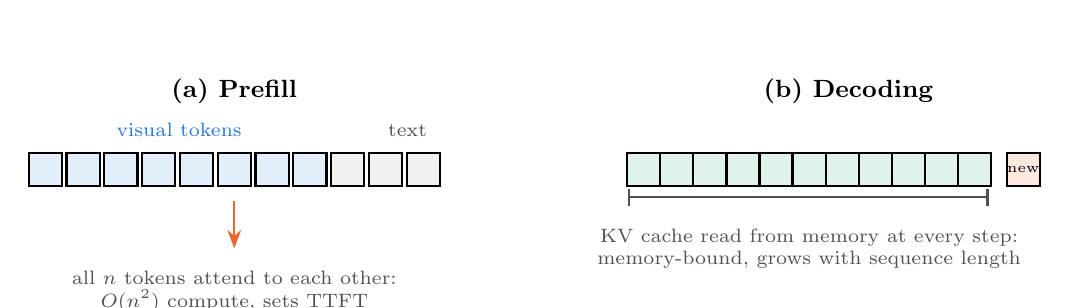
\begin{tikzpicture}[>=Stealth, thick,
  tok/.style={draw, minimum size=0.42cm, inner sep=0pt, font=\tiny},
  lab/.style={font=\small\bfseries},
  note/.style={font=\scriptsize, text=inkgray, align=center}]
\foreach \i in {0,...,7} \node[tok, fill=boxblue] at (\i*0.48,0) {};
\foreach \i in {8,...,10} \node[tok, fill=boxgray] at (\i*0.48,0) {};
\node[lab] at (2.4,1.0) {(a) Prefill};
\draw[->, seriesB] (2.4,-0.4) -- (2.4,-1.0);
\node[note] at (2.4,-1.55) {all $n$ tokens attend to each other:\\ $O(n^2)$ compute, sets TTFT};
\node[font=\scriptsize, text=seriesA] at (1.7,0.5) {visual tokens};
\node[font=\scriptsize, text=inkgray] at (4.6,0.5) {text};
\foreach \i in {0,...,10} \node[tok, fill=boxgreen] at (7.6+\i*0.42,0) {};
\node[tok, fill=boxorange] at (7.6+11*0.42+0.2,0) {new};
\node[lab] at (10.2,1.0) {(b) Decoding};
\draw[|-|, inkgray] (7.4,-0.35) -- (11.98,-0.35);
\node[note] at (9.7,-1.0) {KV cache read from memory at every step:\\ memory-bound, grows with sequence length};
\end{tikzpicture}
\caption{Prefill and decoding phases of VLM inference}
\label{fig:prefill}
\end{figure}

\section{Multimodal Chain-of-Thought and Latent Reasoning}

\paragraph{} \textbf{Chain-of-thought} (CoT) prompting \cite{wei2022} elicits step-by-step reasoning by having a model write out intermediate steps before its answer. Multimodal extensions interleave visual evidence such as image crops, boxes, or tool outputs with these steps, and unified models such as Chameleon and Anole generate interleaved text and images at the cost of pixel-level pretraining \cite{p1}. LLMs can also reason in \textbf{latent space}, replacing some reasoning tokens with continuous hidden-state vectors. The reviewed works combine these ideas: \cite{p2} adds discrete perception tokens as intermediate steps, and \cite{p1} adds continuous latent visual tokens.

\section{Discrete Visual Tokenisation}

\paragraph{} A \textbf{Vector-Quantised Variational Autoencoder} (VQ-VAE) \cite{oord2017} represents an image, or an intrinsic map such as depth, as a grid of discrete codes. An encoder maps the input to a grid of vectors $z_e$, each vector is replaced by its nearest entry in a learned codebook $\{e_k\}_{k=1}^{K}$,
\begin{equation}
z_q=e_{k^{*}},\qquad k^{*}=\arg\min_{k}\big\|z_e-e_k\big\|_2,
\end{equation}
and a decoder reconstructs the input from the codes. The code indices form a short token sequence that a language model can predict like words, which is how \cite{p2} turns depth maps into perception tokens.

\section{Training Paradigms}

\paragraph{} Besides \textbf{supervised fine-tuning} (SFT) with the next-token loss, the reviewed works use \textbf{curriculum learning}, which orders tasks by difficulty to avoid catastrophic forgetting \cite{p2}. \textbf{Distillation} trains a model to match targets produced by another model or encoder, such as image embeddings \cite{p1} or specialist depth predictions \cite{p2,p4}. Finally, \textbf{reinforcement learning} with \textbf{Group Relative Policy Optimisation} (GRPO) \cite{shao2024} samples several responses per question, rewards correct and well-formatted answers, and favours responses that score above the group average, without a separate value network \cite{p1}.

\section{Benchmarks and Evaluation Metrics}

\paragraph{} The reviewed works evaluate on a wide range of benchmarks (Table~\ref{tab:bench}). Accuracy is the main metric for question answering, reasoning, and counting, with CIDEr for captioning and recall at $k$ for retrieval. Efficiency is measured by time-to-first-token, decoding throughput in tokens per second, the share of tokens kept, the reduction in attention floating-point operations (FLOPs), and the reduction in KV-cache size \cite{p3}.

{\renewcommand{\arraystretch}{1.15}
\begin{table}[htbp]
\centering
\caption{Benchmarks used in the reviewed works}\label{tab:bench}
\small
\begin{tabularx}{\textwidth}{|>{\raggedright\arraybackslash}p{3.0cm}|X|p{1.4cm}|}
\hline
\textbf{Category} & \textbf{Benchmarks} & \textbf{Used in} \\ \hline
Spatial reasoning & VSP spatial reasoning and planning, BLINK-Jigsaw, SAT, COMT geometry & \cite{p1} \\ \hline
Depth and counting & BLINK relative depth, HardBLINK, CV-Bench, SEED-Bench, BLINK counting & \cite{p2} \\ \hline
Image understanding & VQAv2, GQA, TextVQA, ChartQA, MME, MMBench, MMVet, SEED & \cite{p3,p4} \\ \hline
Video understanding & Video-MME, EgoSchema, MSVD, ActivityNet, MLVU & \cite{p3,p4} \\ \hline
Encoder evaluation & Zero-shot classification, Kinetics, Flickr30K and COCO retrieval & \cite{p4} \\ \hline
\end{tabularx}
\end{table}}

\section{Taxonomy of Approaches}

\paragraph{} Figure~\ref{fig:taxonomy} organises the reviewed works by the limitation of VLMs they address. Two works enrich \emph{reasoning} with new kinds of visual tokens, one improves \emph{efficiency}, and one improves the \emph{data and pretraining} from which visual understanding is learned.

\begin{figure}[htbp]
\centering
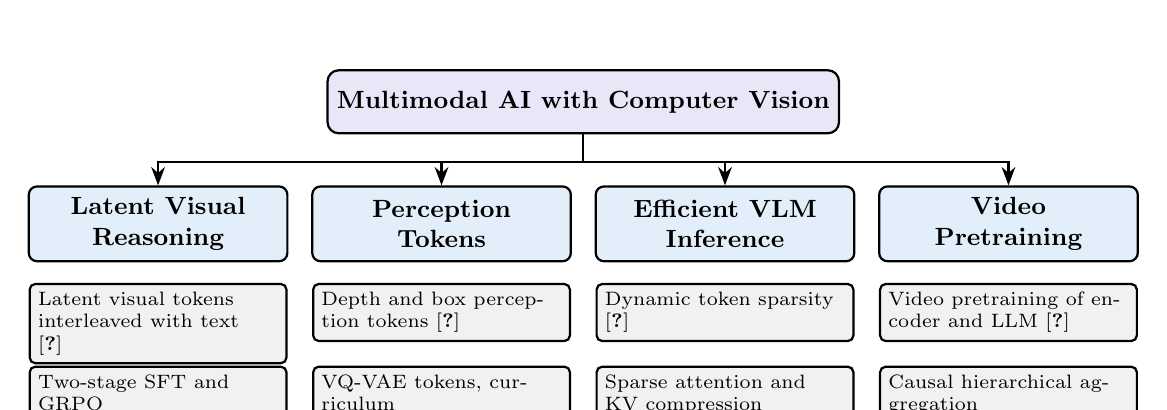
\begin{tikzpicture}[>=Stealth, thick,
  root/.style={draw, rounded corners=4pt, fill=boxviolet, font=\small\bfseries, minimum width=5.6cm, minimum height=0.8cm, align=center},
  cat/.style={draw, rounded corners=3pt, fill=boxblue, font=\small\bfseries, text width=3.05cm, align=center, minimum height=0.95cm},
  leaf/.style={draw, rounded corners=2pt, fill=boxgray, font=\scriptsize, text width=3.05cm, align=left, inner sep=3pt}]
\node[root] (r) at (5.4,0) {Multimodal AI with Computer Vision};
\foreach \x/\n/\t in {0/a/Latent Visual\\ Reasoning,3.6/b/Perception\\ Tokens,7.2/c/Efficient VLM\\ Inference,10.8/d/Video\\ Pretraining} {
  \node[cat] (\n) at (\x,-1.55) {\t};
  \draw[->] (r.south) -- ++(0,-0.35) -| (\n.north);
}
\node[leaf, anchor=north] at (0,-2.3) {Latent visual tokens interleaved with text \cite{p1}};
\node[leaf, anchor=north] at (0,-3.35) {Two-stage SFT and GRPO};
\node[leaf, anchor=north] at (3.6,-2.3) {Depth and box perception tokens \cite{p2}};
\node[leaf, anchor=north] at (3.6,-3.35) {VQ-VAE tokens, curriculum};
\node[leaf, anchor=north] at (7.2,-2.3) {Dynamic token sparsity \cite{p3}};
\node[leaf, anchor=north] at (7.2,-3.35) {Sparse attention and KV compression};
\node[leaf, anchor=north] at (10.8,-2.3) {Video pretraining of encoder and LLM \cite{p4}};
\node[leaf, anchor=north] at (10.8,-3.35) {Causal hierarchical aggregation};
\end{tikzpicture}
\caption{Taxonomy of the reviewed approaches}
\label{fig:taxonomy}
\end{figure}

% ================= CHAPTER 3: LITERATURE SURVEY =================
\chapter{Literature Survey}

\paragraph{} This chapter reviews the four works in detail. For each, it describes the problem and motivation, the method, the experimental setup and results, and closes with a short discussion of strengths and limitations.

% ---------------------------------------------------------------
\section{Machine Mental Imagery: Empower Multimodal Reasoning with Latent Visual Tokens}

\paragraph{} The base paper, by Yang, Yu, Chen, Shen, and Gan \cite{p1}, from the University of Massachusetts Amherst, MIT, and the MIT-IBM Watson AI Lab, introduces \textbf{Mirage}, a framework that lets a VLM reason with compact latent visual tokens interleaved with ordinary text.

\subsection{Problem Statement and Motivation}

\paragraph{} VLMs decode only text, so they must \emph{verbalise} visual reasoning. This limits them on tasks such as spatial planning and jigsaw puzzles, where people instead picture how pieces fit or how a path unfolds. Recent unified models can generate images while reasoning, but heavy image-generation pretraining tends to degrade reasoning, and their image decoders cannot produce interleaved trajectories tied to the input images \cite{p1}. Imagery theory suggests that humans do not imagine photorealistic pictures; they build simplified \emph{mental images} that keep only task-relevant cues. Mirage asks whether a VLM can do the same by reasoning directly in its latent visual embedding space, without producing pixels (Figure~\ref{fig:p1_examples}).

\begin{figure}[htbp]
\centering
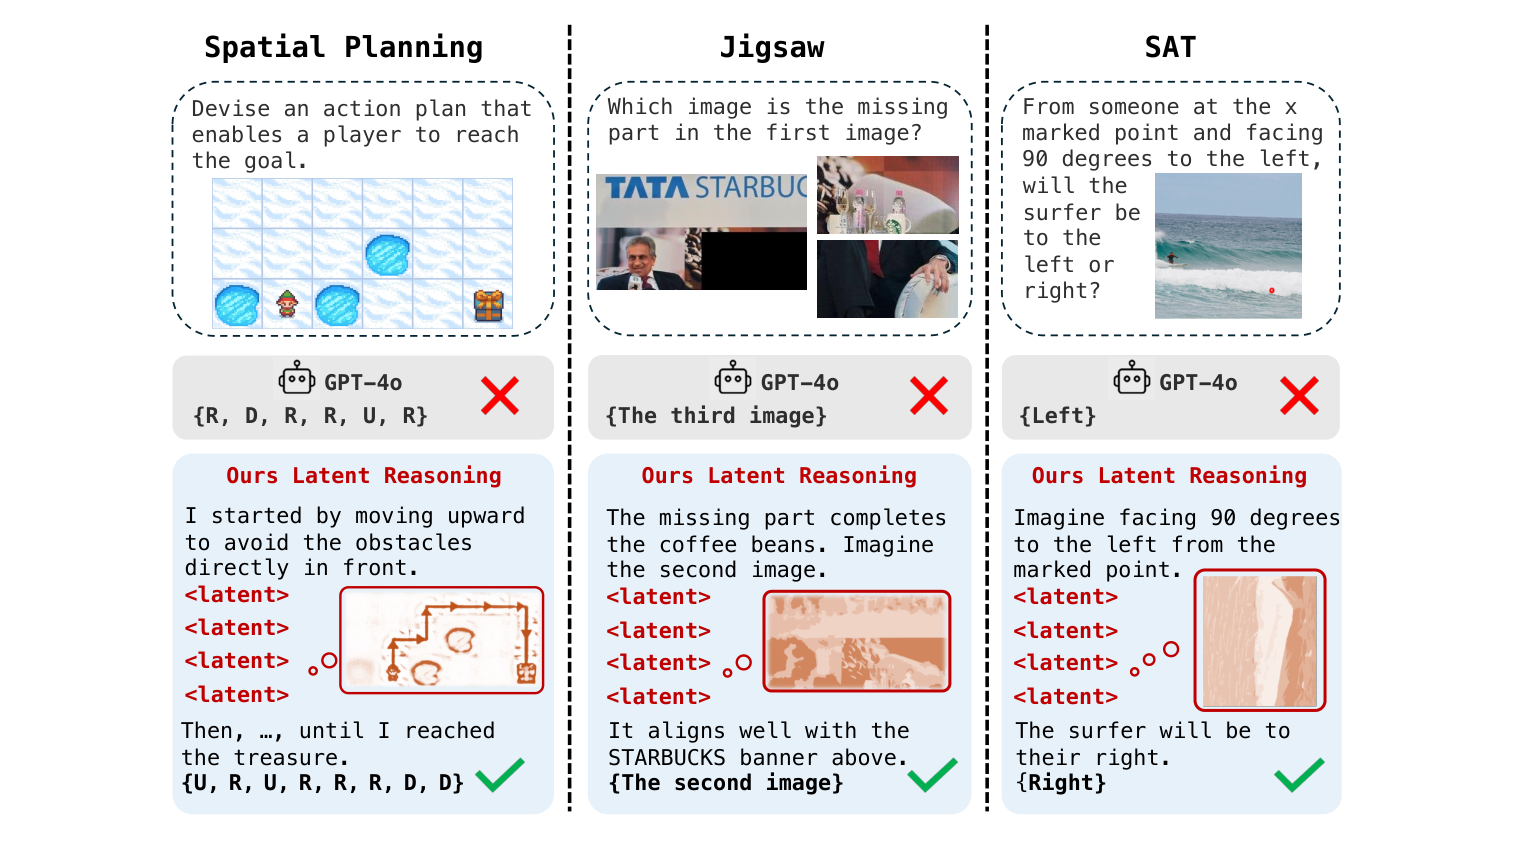
\includegraphics[width=0.86\textwidth]{figs/p1_examples.png}
\caption{Mirage reasoning examples with latent visual tokens \cite{p1}}
\label{fig:p1_examples}
\end{figure}

\subsection{Method}

\paragraph{} \textbf{Data synthesis.} Each training question $x$ with answer $y$ is paired with a task-specific \emph{helper image} $I$ that contains exactly the visual cue needed: for maze navigation, the start map with the correct path drawn in red arrows; for jigsaw, a candidate piece placed beside the reference image; for spatial-aptitude questions, a scene rendered by a fine-tuned CogVideoX-5B video model. A large reasoning VLM, Qwen2.5-VL-32B, is then prompted to write a step-by-step solution that incorporates the helper image, producing a trajectory $o=o_{\mathrm{pre}}\oplus I\oplus o_{\mathrm{post}}$ in which the image splits the text into a part before and a part after it \cite{p1}.

\paragraph{} \textbf{Stage 1: joint supervision.} Rather than asking the model to generate the helper image, Mirage passes it through the VLM to obtain patch features $\{e_1,\dots,e_n\}$ and compresses them by average pooling into $k$ salient vectors $\{\hat{e}_1,\dots,\hat{e}_k\}$. The model is trained to produce $o_{\mathrm{pre}}$, then to output these $k$ vectors as its last-layer hidden states at the latent positions, and then to produce $o_{\mathrm{post}}$. The latent tokens are supervised with a cosine loss,
\begin{equation}
\mathcal{L}_{\mathrm{visual}}=\sum_{j=1}^{k}\ell_{\cos}\big(\hat{e}_j,\;g_\theta(o_{\mathrm{pre}},\hat{e}_{1:j-1})\big),
\end{equation}
and the text with the usual cross-entropy loss $\mathcal{L}_{\mathrm{text}}$, giving $\mathcal{L}_1=\mathcal{L}_{\mathrm{visual}}+\gamma\,\mathcal{L}_{\mathrm{text}}$. This anchors the latent tokens in the visual subspace while teaching the model to weave them into its thoughts (Figure~\ref{fig:p1_pipeline}).

\begin{figure}[htbp]
\centering
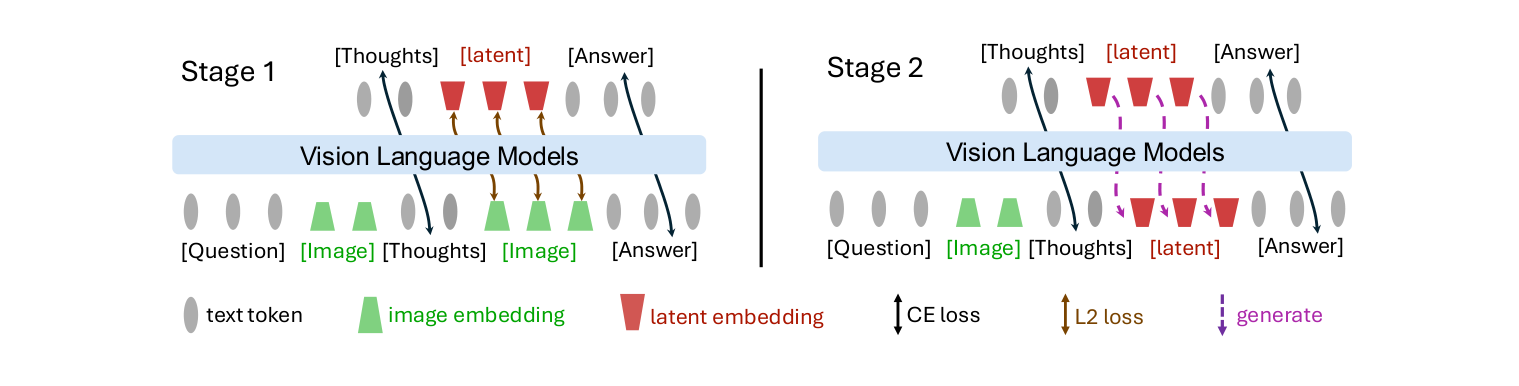
\includegraphics[width=0.92\textwidth]{figs/p1_pipeline.png}
\caption{Two-stage training pipeline of Mirage \cite{p1}}
\label{fig:p1_pipeline}
\end{figure}

\paragraph{} \textbf{Stage 2: text-only supervision.} Forcing latent tokens to reconstruct image embeddings can over-constrain the model and divert capacity from answering correctly. In the second stage, the cosine loss is removed: the model generates its own latent tokens autoregressively, $e_j=f_\theta(x,o_{\mathrm{pre}},e_{<j})$, and only the text tokens are supervised. Because the latent tokens are continuous, gradients from the text loss flow back through them, so they adapt freely within the learned visual subspace and act as priors for the text that follows \cite{p1}.

\paragraph{} \textbf{Reinforcement learning.} Finally, the model is refined with GRPO \cite{shao2024}, sampling several responses per question. The reward is 1 for a correct final answer and an extra 0.1 when the reasoning is enclosed in think tags and the answer is given in the required boxed format; gradients again flow through the latent tokens \cite{p1}.

\subsection{Experimental Setup}

\paragraph{} The default base model is Qwen2.5-VL 7B with $k=4$ latent tokens and loss coefficient $\gamma=0.1$. Four benchmarks are used: \textbf{VSP}, with spatial-reasoning and spatial-planning tasks in a simulated maze; \textbf{BLINK-Jigsaw}; \textbf{SAT}, with static and dynamic spatial relations; and the geometry subset of \textbf{COMT}. For each task, 1k examples are used for fine-tuning and 1k for reinforcement learning. Baselines include zero-shot and directly fine-tuned models, CoT fine-tuning with and without GRPO, unified models that generate images (Anole and MVoT), and interleaved reasoning models such as AURORA \cite{p2}, ViGoRL, MindJourney, and MINT-CoT \cite{p1}.

\subsection{Results and Analysis}

\paragraph{} Table~\ref{tab:p1_vsp} shows average accuracy on the two VSP tasks. Latent visual tokens improve both reasoning styles: Mirage beats direct fine-tuning by 3 points on spatial reasoning and CoT fine-tuning by 11 points on spatial planning, and GRPO adds a further 2 points. Models that explicitly generate images perform poorly; even after fine-tuning on the same data, AURORA reaches 0.71 and 0.13, which the authors attribute to the overhead of image generation \cite{p1}. With the smaller Qwen2.5-VL 3B, Mirage reaches 0.85 on Jigsaw, 0.89 on synthetic SAT, and 0.64 on real SAT, against 0.80, 0.83, and 0.55 for direct fine-tuning, and on COMT geometry it scores 0.77 against 0.72 for MINT-CoT, which was trained on large-scale mathematics data.

{\renewcommand{\arraystretch}{1.12}
\begin{table}[htbp]
\centering
\caption{Mirage on the VSP benchmark}\label{tab:p1_vsp}
\small
\begin{tabular}{|l|c|c|}
\hline
\textbf{Method (Qwen2.5-VL 7B)} & \textbf{Spatial reasoning (avg.)} & \textbf{Spatial planning (avg.)} \\ \hline
Zero-shot & 0.32 & 0.06 \\ \hline
Direct SFT & 0.83 & 0.72 \\ \hline
CoT SFT & 0.84 & 0.47 \\ \hline
CoT SFT + GRPO & 0.85 & 0.51 \\ \hline
Anole / MVoT / AURORA & 0.52 / 0.61 / 0.71 & 0.01 / 0.11 / 0.13 \\ \hline
Mirage (direct) & 0.86 & \textbf{0.76} \\ \hline
Mirage (CoT) & 0.87 & 0.58 \\ \hline
Mirage (CoT) + GRPO & \textbf{0.89} & 0.60 \\ \hline
\end{tabular}
\end{table}}

\paragraph{} \textbf{Ablations.} Removing Stage 1 lowers spatial-planning accuracy from 0.58 to 0.52, because ungrounded latent vectors drift to unhelpful regions of the embedding space; removing Stage 2 leaves the latent tokens over-constrained and drops it to 0.21, so both stages are necessary. Performance is stable for $k$ between 2 and 6 latent tokens but falls by about 13 points at $k=8$, consistent with error accumulation over longer latent sequences, and every tested value of $\gamma$ still exceeds 80\% accuracy after Stage 2 \cite{p1}.

\paragraph{} \textbf{Latent behaviour.} Supplying the helper images directly as input lets models reach nearly 100\% on the VSP tasks, confirming that the synthesised cues are informative and indicating an upper bound for latent reasoning. A t-SNE projection shows that Mirage's latent tokens form a compact cloud just outside the cluster of visual embeddings and far from the text embeddings: they remain visual in character but are shifted by Stage 2 towards what helps answer generation, echoing how mental imagery abstracts rather than reproduces what is seen \cite{p1}.

\subsection{Discussion}

\paragraph{} Mirage's main strength is that it adds visual thinking to a VLM cheaply: four latent vectors replace a generated image, no image decoder is needed, and the approach transfers from 7B to 3B models. Its two-stage design is well supported by ablations. Its limitations are the reliance on synthesised helper images and reasoning traces, which can be noisy---especially for SAT, whose helper images come from a video generator without ground truth---and evaluation on four spatial benchmarks with 1k training examples each. On VSP planning, fine-tuning on reasoning traces also underperforms fine-tuning on answers alone, showing that explicit reasoning does not always help perception-heavy tasks.

% ---------------------------------------------------------------
\section{Perception Tokens Enhance Visual Reasoning in Multimodal Language Models}

\paragraph{} Bigverdi, Luo, Hsieh, Shen, Chen, Shapiro, and Krishna \cite{p2}, from the University of Washington and Google Research, introduce \textbf{perception tokens} and \textbf{AURORA}, a training method that teaches multimodal language models to produce and reason over them.

\subsection{Problem Statement and Motivation}

\paragraph{} MLMs still fail at basic perception tasks where specialist vision models excel. Deciding which of several marked points is closest to the camera is hard to reason about in words but easy with a depth map, and counting objects is easier with their bounding boxes. Fine-tuning MLMs on such tasks generalises poorly, and calling external depth estimators or detectors is compute- and memory-intensive and fragile \cite{p2}. The authors therefore let the model generate intrinsic image representations itself, as intermediate reasoning steps akin to chain-of-thought \cite{wei2022}: for example, ``The depth map is $\langle$perception tokens$\rangle$. Therefore, point D is closest to the camera.''

\subsection{Perception Tokens and Training}

\paragraph{} The model's vocabulary $V$ is expanded to $V'=V\cup V_{\mathrm{aux}}$ with auxiliary perception tokens. Two kinds are used. \textbf{Pixel-level tokens} encode depth maps: a VQ-VAE \cite{oord2017} with a 128-entry codebook compresses each $320\times320$ depth map into a $10\times10$ grid, giving 100 tokens drawn from 128 depth tokens plus start and end markers, 130 new tokens in all; it is trained on pseudo-depth maps of ADE20k images produced by Depth Anything. \textbf{Structured tokens} encode bounding boxes: images are resized to $336\times336$ and 336 coordinate tokens are added, so a box is written as four tokens $(x_1,y_1,x_2,y_2)$ \cite{p2}.

\paragraph{} To learn to \emph{predict} perception tokens, AURORA distils from specialist models: if a specialist gives a target distribution $q_i$ over its tokens and $\mathcal{M}$ maps them to auxiliary tokens, the loss is
\begin{equation}
\ell_{\mathrm{dist}}=-\sum_{i}q_i\log p_{\mathcal{M}(i)},
\end{equation}
optionally combined with a reconstruction loss $\ell_{\mathrm{rec}}=\|g(T)-f\|_2^2$ through a lightweight decoder $g$ that maps a token set $T$ back to its target feature $f$. To learn to \emph{reason} with them, training mixes three subsets of increasing difficulty---generating perception tokens, answering with chain-of-thought through perception tokens, and answering directly---and samples task $t$ of difficulty $d_t$ at step $s$ with a curriculum
\begin{equation}
p(d_t,s)=\frac{\exp\big(-d_t/\tau(s)\big)}{\sum_{i=1}^{m}\exp\big(-d_i/\tau(s)\big)},\qquad \tau(s)=\frac{\tau_0}{1+\lambda\cdot s/S},
\end{equation}
which shifts sampling between tasks over training to avoid catastrophic forgetting (Figure~\ref{fig:p2_framework}). At inference, constrained decoding restricts sampling to auxiliary tokens at the steps where they are expected \cite{p2}.

\begin{figure}[htbp]
\centering
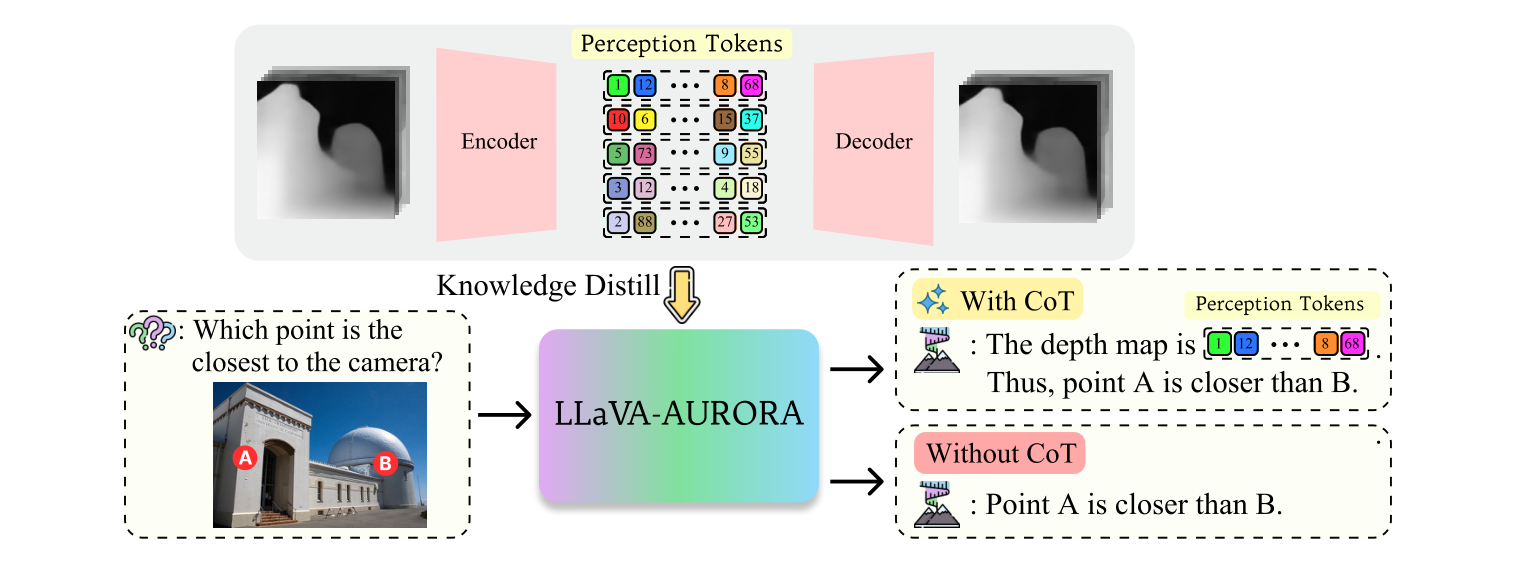
\includegraphics[width=0.80\textwidth]{figs/p2_framework.png}
\caption{AURORA training framework \cite{p2}}
\label{fig:p2_framework}
\end{figure}

\subsection{Experimental Setup}

\paragraph{} AURORA is applied to LLaVA 1.5 13B, giving \textbf{LLaVA-AURORA}. For relative depth, training uses 20k ADE20k depth-generation examples and 500 images with 2--5 markers for chain-of-thought and direct answers; evaluation uses BLINK relative depth and \textbf{HardBLINK}, harder variants with 3, 4, and 5 markers placed at mid-height to remove height cues. For counting, training uses 5k LVIS images with 0--15 objects and 250 images for reasoning; evaluation uses CV-Bench, SEED-Bench, and BLINK counting, all without multiple-choice options. Baselines include LLaVA fine-tuned on the same direct-answer data, LLaVA-OneVision, GPT-4o, GPT-4 Turbo, and GPT-4 Turbo with tools \cite{p2}.

\subsection{Results and Analysis}

\paragraph{} Table~\ref{tab:p2_res} summarises the results. On relative depth, LLaVA-AURORA averages 61.6\% over BLINK and HardBLINK, against 55.2\% for the fine-tuned baseline, and its advantage grows with the number of points, reaching 54.8\% on five points against 41.1\%. It also surpasses GPT-4o and GPT-4 Turbo, even when the latter is given ground-truth depth maps. On counting, it improves on the fine-tuned baseline by 11.3 points on CV-Bench and 8.3 on SEED-Bench, and on the base model by 10.8 on BLINK, where the fine-tuned baseline collapses \cite{p2}. Decoded depth maps resemble the ground truth (Figure~\ref{fig:p2_depth}), and their programmatic relative-depth accuracy, 79.2\% on average, exceeds Unified-IO's 74.4\%.

{\renewcommand{\arraystretch}{1.12}
\begin{table}[htbp]
\centering
\caption{AURORA on relative depth and counting}\label{tab:p2_res}
\small
\setlength{\tabcolsep}{4pt}
\begin{tabular}{|l|c|c|c|c|c|}
\hline
\textbf{Model} & \textbf{Depth avg.} & \textbf{Depth 5-pt} & \textbf{CV-Bench} & \textbf{SEED} & \textbf{BLINK} \\ \hline
LLaVA 1.5 13B & 39.1 & 29.0 & 40.9 & 52.2 & 35.0 \\ \hline
Fine-tuned LLaVA & 55.2 & 41.1 & 44.7 & 46.3 & 0.2 \\ \hline
LLaVA-OneVision & 53.4 & 44.3 & 34.4 & 31.7 & 35.8 \\ \hline
GPT-4o & 49.6 & 36.3 & 70.2 & 64.6 & 47.5 \\ \hline
GPT-4 Turbo + Tool & 49.6 & 26.6 & 48.6 & 29.9 & 26.7 \\ \hline
LLaVA-AURORA & \textbf{61.6} & \textbf{54.8} & 56.0 & 54.6 & 45.8 \\ \hline
\end{tabular}
\end{table}}

\begin{figure}[htbp]
\centering
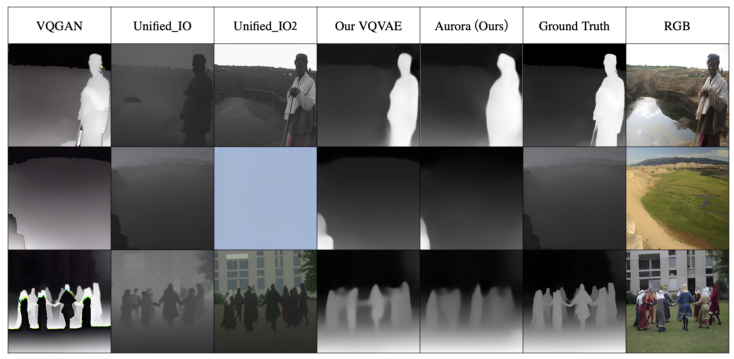
\includegraphics[width=0.62\textwidth]{figs/p2_depthmaps.png}
\caption{Depth maps decoded from AURORA perception tokens \cite{p2}}
\label{fig:p2_depth}
\end{figure}

\subsection{Discussion}

\paragraph{} AURORA shows that a single MLM can learn to produce useful intermediate perception without external tools, and that chain-of-thought over such tokens generalises across benchmarks better than plain fine-tuning. Its framework is extensible to other intrinsics such as segmentation masks or poses. Its limitations are the narrow evaluation, two tasks on one base model, a slightly lower score than the fine-tuned baseline on the original two-point BLINK depth task (64.5\% against 68.5\%), and counting accuracy still below closed-source models such as GPT-4o. Mirage \cite{p1} later found that explicit token generation of this kind is less effective for interleaved spatial reasoning than compact latent tokens.

% ---------------------------------------------------------------
\section{ZipVL: Accelerating Vision-Language Models through Dynamic Token Sparsity}

\paragraph{} He, Chen, Liu, Shao, Zhou, Zhang, and Zhuang \cite{p3}, from Zhejiang University, the Shanghai AI Laboratory, the University of Adelaide, and Monash University, present \textbf{ZipVL}, an inference framework that speeds up both phases of large VLM (LVLM) generation with a single, dynamically chosen set of important tokens.

\subsection{Problem Statement and Motivation}

\paragraph{} High-resolution images and videos produce very long token sequences---a 128-frame video becomes over 18,000 tokens in the LongVA model. The prefill phase then suffers from quadratic attention cost and a long time-to-first-token, and the decoding phase from repeatedly reading a large KV cache \cite{p3}. Visual content is highly redundant, so attention maps in LVLMs are sparse, but their sparsity varies across layers and tasks (Figure~\ref{fig:p3_attn}). Existing methods tackle only one bottleneck, rely on predefined sparse patterns that need custom GPU kernels, or keep a fixed share of tokens---FastV, for example, drops half of the visual tokens after the second layer and degrades on hard tasks such as ChartQA.

\begin{figure}[htbp]
\centering
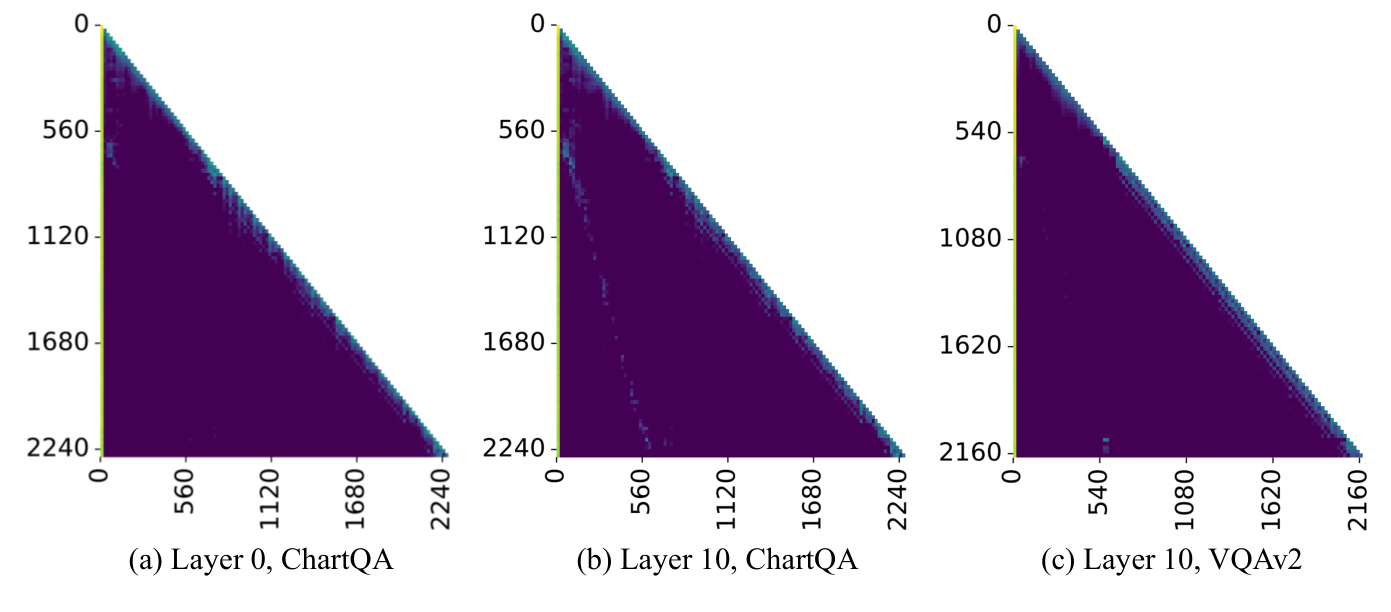
\includegraphics[width=0.78\textwidth]{figs/p3_attnmaps.png}
\caption{Attention maps across layers and tasks in an LVLM \cite{p3}}
\label{fig:p3_attn}
\end{figure}

\subsection{Method}

\paragraph{} \textbf{Layer-wise adaptive ratio.} In each layer, ZipVL sums the attention each token receives, $a_j=\sum_{c=1}^{n}A_{c,j}$, sorts these scores, and keeps the smallest number of tokens that preserves a fraction $\tau$ of the total attention:
\begin{equation}
p=\min\Big\{p\in\mathbb{Z}\;\Big|\;\sum_{j=1}^{p}a_{\mathrm{sorted}(j)}\ge\tau\times n\Big\},
\end{equation}
where the total is $n$ because every row of $A$ sums to one. Simple tasks concentrate attention on few tokens and get a small $p$; harder tasks spread attention and get a larger $p$, so the ratio adapts to each layer and task without hand-set hyperparameters (Figure~\ref{fig:p3_ratio}) \cite{p3}.

\paragraph{} \textbf{Important-token selection.} Tokens are ranked by their \emph{normalised} attention score, $\tilde{a}_j=\sum_{c}A_{c,j}/\mathrm{nnz}(A_{:,j})$, which corrects for the causal mask giving early tokens more attention, and the top $p$ form the important set $T$. In the \textbf{prefill} phase, attention is computed only among the important tokens using standard FlashAttention, and the outputs of the other tokens are padded; in the \textbf{decoding} phase, only the important tokens' keys and values are kept in the cache. Because FlashAttention never materialises the full attention matrix, the scores are approximated from a small, fixed set of probe tokens (Figure~\ref{fig:p3_overview}, Algorithm~\ref{alg:p3}) \cite{p3}.

\begin{figure}[htbp]
\centering
\begin{subfigure}[b]{0.55\textwidth}\centering
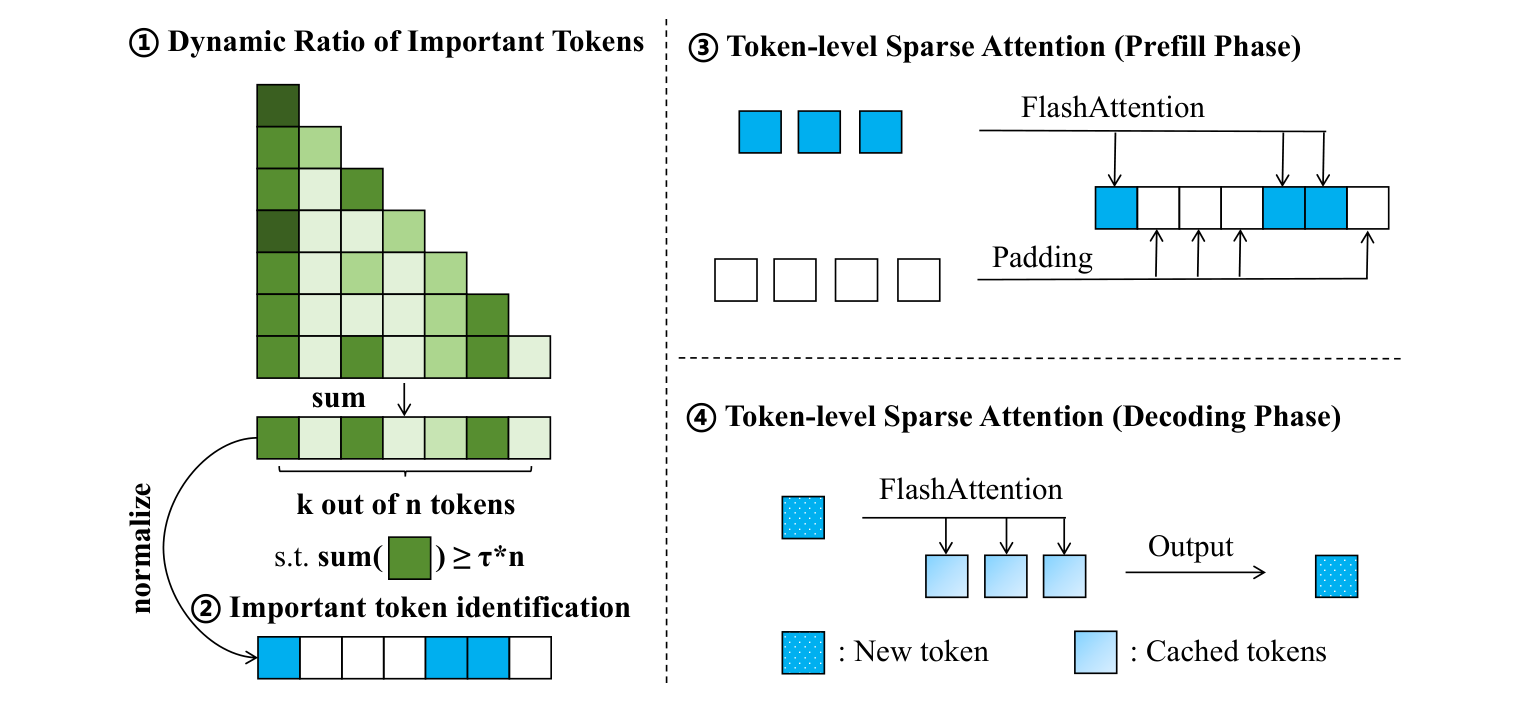
\includegraphics[width=\linewidth]{figs/p3_overview.png}
\caption{Framework overview}\label{fig:p3_overview}
\end{subfigure}\hfill
\begin{subfigure}[b]{0.41\textwidth}\centering
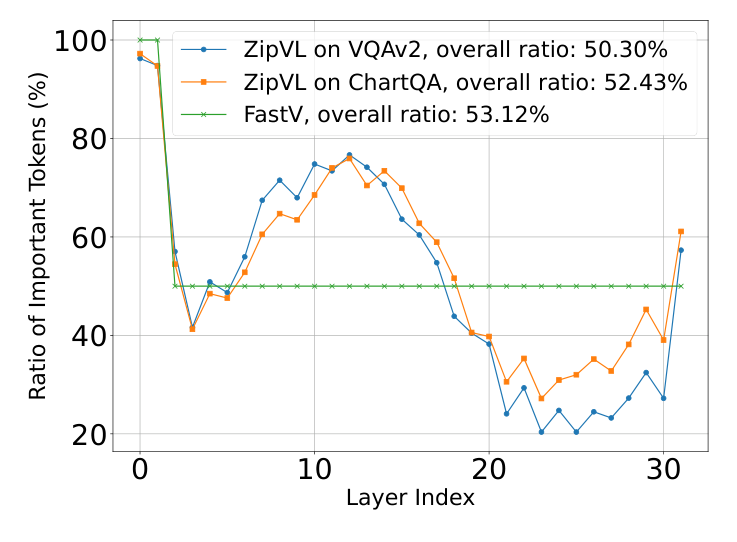
\includegraphics[width=\linewidth]{figs/p3_layerratio.png}
\caption{Important-token ratio per layer}\label{fig:p3_ratio}
\end{subfigure}
\caption{The ZipVL framework and its layer-wise token ratio \cite{p3}}
\label{fig:p3_fw}
\end{figure}

\begin{algorithm}[htbp]
\caption{Prefill phase of ZipVL (adapted from \cite{p3})}\label{alg:p3}
\begin{algorithmic}[1]
\Require input embeddings $X$; attention-retention threshold $\tau$
\State Compute $Q$, $K$, $V$ from $X$
\State Compute attention scores $A'$ for a small set of probe queries against all keys
\State Find the number of important tokens $p$ from the sorted accumulated scores
\State Compute normalised scores $\tilde{a}_j$ and select $T=\mathrm{topk}(\tilde{a},p)$
\State $O\gets\mathrm{FlashAttention}(Q[T],K[T],V[T])$; pad outputs of the remaining tokens
\State Keep only $K[T]$ and $V[T]$ in the KV cache for decoding
\end{algorithmic}
\end{algorithm}

\subsection{Experimental Setup}

\paragraph{} Image understanding is evaluated with LLaVA-1.5-7B, LLaVA-Next-7B, and LLaVA-Next-13B on VQAv2, TextVQA, GQA, MME, and ChartQA, against FastV and HiRED. Video understanding is evaluated with LongVA-7B on Video-MME with 64 and 128 frames, against MInference, QK-sparse, and FastV. Latency and throughput are measured for LLaVA-Next-13B on an NVIDIA A100 GPU \cite{p3}.

\subsection{Results and Analysis}

\paragraph{} \textbf{Accuracy.} Table~\ref{tab:p3_img} shows results on LLaVA-Next-13B. With $\tau=0.975$, ZipVL keeps only 36.8\% of tokens yet stays within 0.5 points of the full model on VQAv2 and matches it on MME, while FastV, keeping 53.1\%, loses much more, especially on ChartQA. ZipVL outperforms FastV on nearly all benchmarks across the three models, and HiRED, which ignores the text prompt when choosing patches, loses accuracy, especially at low token ratios. On Video-MME with 128 frames, ZipVL matches the full model's 52.6\% while cutting attention FLOPs by 82.3\% and the KV cache by 57.9\%; a fixed ratio with the same overall sparsity reaches only 51.1\% \cite{p3}.

{\renewcommand{\arraystretch}{1.12}
\begin{table}[htbp]
\centering
\caption{ZipVL on image benchmarks with LLaVA-Next-13B}\label{tab:p3_img}
\small
\begin{tabular}{|l|c|c|c|c|c|c|}
\hline
\textbf{Method} & \textbf{Tokens kept} & \textbf{VQAv2} & \textbf{ChartQA} & \textbf{TextVQA} & \textbf{GQA} & \textbf{MME} \\ \hline
Full attention & 100\% & 80.9 & 66.2 & 66.9 & 65.7 & 1570 \\ \hline
FastV & 53.1\% & 76.8 & 51.6 & 59.7 & 62.9 & 1555 \\ \hline
HiRED & 40\% & 79.3 & 53.7 & 65.2 & 64.1 & 1570 \\ \hline
ZipVL ($\tau=0.96$) & 30.6\% & 79.7 & 57.8 & 63.6 & 64.3 & 1551 \\ \hline
ZipVL ($\tau=0.975$) & 36.8\% & 80.4 & 58.5 & 64.9 & 64.8 & 1574 \\ \hline
\end{tabular}
\end{table}}

\paragraph{} \textbf{Efficiency.} Figure~\ref{fig:p3_ttft} plots the time-to-first-token. For short inputs ZipVL matches FlashAttention, but as inputs grow the attention module dominates and the savings rise, reaching a 2.3 times reduction at 128K tokens (20.57 s against 48.01 s). MInference is slower than FlashAttention below 32K tokens, and FastV, which needs full attention scores, runs out of memory beyond 8K. Because the smaller KV cache allows larger batches, ZipVL also raises decoding throughput by about 2.8 times at 16K tokens (40.87 against 14.10 tokens/s) and keeps decoding at 32K and 64K, where the baselines run out of memory. Applied to KV-cache quantisation of LLaMA3-8B, the adaptive ratio also gives a higher compression ratio than ZipCache (6.18 against 4.69 times) with better accuracy \cite{p3}.

\begin{figure}[htbp]
\centering
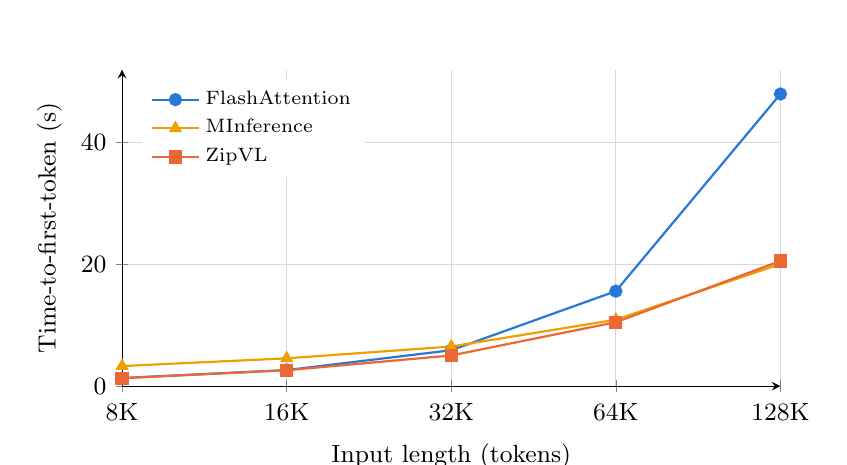
\begin{tikzpicture}
\begin{axis}[width=0.82\textwidth, height=5.6cm, xmode=log, log basis x=2, xtick={8,16,32,64,128}, xticklabels={8K,16K,32K,64K,128K},
  xlabel={Input length (tokens)}, ylabel={Time-to-first-token (s)}, ymin=0, ymax=52, grid=major, grid style={gridgray}, axis lines=left,
  legend style={at={(0.03,0.97)}, anchor=north west, font=\scriptsize, draw=none, fill=white, cells={anchor=west}},
  tick label style={font=\small}, label style={font=\small}]
\addplot[seriesA, thick, mark=*] coordinates {(8,1.33) (16,2.64) (32,5.90) (64,15.61) (128,48.01)};
\addplot[seriesD, thick, mark=triangle*] coordinates {(8,3.30) (16,4.57) (32,6.51) (64,10.92) (128,20.08)};
\addplot[seriesB, thick, mark=square*] coordinates {(8,1.31) (16,2.61) (32,5.04) (64,10.51) (128,20.57)};
\legend{FlashAttention, MInference, ZipVL}
\end{axis}
\end{tikzpicture}
\caption{Time-to-first-token versus input length (data from \cite{p3})}
\label{fig:p3_ttft}
\end{figure}

\subsection{Discussion}

\paragraph{} ZipVL's strengths are that one signal---the attention distribution---drives both sparse prefill and KV-cache eviction, that it works with standard FlashAttention without custom kernels, and that its ratio adapts automatically to layers, tasks, and models. Its limitations are that only attention is sparsified while the MLP layers stay dense, that probe-based score approximation adds overhead at short lengths, and that hard tasks such as ChartQA still lose several points; the speed-ups appear mainly for long inputs.

% ---------------------------------------------------------------
\section{Learning Beyond Still Frames: Scaling Vision-Language Models with Video}

\paragraph{} Zhang, Li, Liu, and Yue \cite{p4}, from CUHK, UCAS, CASIA, and the Shanghai AI Laboratory, propose \textbf{LLaVA-Prime}, which adds large-scale video pretraining to the LLaVA recipe to improve both image and video understanding.

\subsection{Problem Statement and Motivation}

\paragraph{} VLMs depend on high-quality image-text pairs, which are expensive to create, and even good image data captures isolated moments with no temporal context, limiting understanding of motion, events, and causality in video. Videos offer richer visual information, because consecutive frames show how scenes evolve, and their captions are longer and more detailed, which encourages finer vision-language alignment. Video, however, is costly to process and requires strict temporal causality \cite{p4}.

\subsection{Method}

\paragraph{} Starting from LLaVA-1.5 with a 1-billion-parameter ViT-g vision encoder and the Qwen2-7B LLM, LLaVA-Prime trains in four stages (Figure~\ref{fig:p4_fw}). \textbf{Stage I} pretrains the vision encoder on video-caption pairs from Panda-70M with the contrastive InfoNCE loss, feeding four key frames reshaped into a single 12-channel input. \textbf{Stage II} pretrains the LLM on interleaved video and text tokens with the next-token loss, stabilised by EVE's patch-aligning layer, and distils the Stage I encoder's features into the LLM's vision tokens with a token-wise squared error,
\begin{equation}
\mathcal{L}_{\mathrm{distill}}=\frac{1}{N_v}\sum_{i=1}^{N_v}\big\|z_{v,i}-e_{v,i}\big\|_2^2,
\end{equation}
where $z_v$ and $e_v$ are the encoder and LLM representations. \textbf{Stage III} trains on joint image-video-text data with the new aggregation module, and \textbf{Stage IV} performs visual instruction tuning with the encoder frozen \cite{p4}.

\begin{figure}[htbp]
\centering
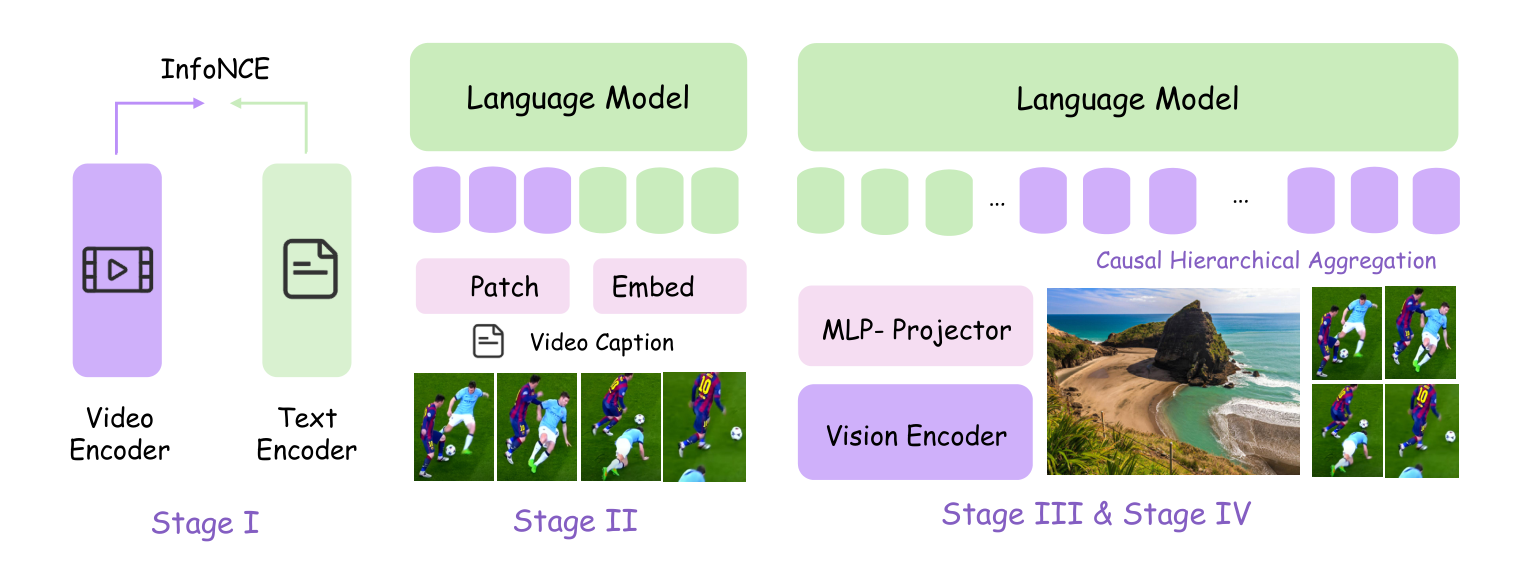
\includegraphics[width=0.82\textwidth]{figs/p4_framework.png}
\caption{The four-stage LLaVA-Prime framework \cite{p4}}
\label{fig:p4_fw}
\end{figure}

\paragraph{} \textbf{Causal Hierarchical Aggregation} (CHA) lets the same image encoder process video while keeping the number of video tokens equal to that of an image. Following run-length tokenisation, a video is represented by its first frame $x_v^0$ and the differences between consecutive frames, $\Delta x_v^{i-1,i}=x_v^{i}-x_v^{i-1}$. A causal 1D convolution aggregates these over time so that each step depends only on the past,
\begin{equation}
z_v^0=w\cdot x_v^0,\qquad z_v^i=z_v^{i-1}\cdot M_i\cdot w\cdot\Delta x_v^{i-1,i},
\end{equation}
and several dilated, large-kernel causal convolutions---dilations 1, 3, 5, and 7 with kernel sizes 13, 13, 9, and 7---build hierarchical temporal receptive fields, compressing $N_v\times T$ video tokens to $N_v$ \cite{p4}.

\subsection{Experimental Setup}

\paragraph{} LLaVA-Prime-7B is trained like LLaVA-OneVision-7B plus 32M Panda-70M video samples (about 25B video tokens at one frame per second), and LLaVA-Prime-72B with 128M samples (about 100B video tokens), on 512 NVIDIA A100 GPUs for two weeks. The encoder is evaluated on zero-shot classification over 27 datasets, Kinetics video recognition, and Flickr30K and COCO retrieval; the full model on image benchmarks such as GQA, VQAv2, MME, MMBench, MMVet, and SEED, and on video benchmarks such as MSVD, ActivityNet, EgoSchema, Video-MME, and MLVU \cite{p4}.

\subsection{Results and Analysis}

\paragraph{} \textbf{Scaling.} Increasing video pretraining data from 2M to 128M samples steadily improves image and video understanding (Figure~\ref{fig:p4_scale}): general image benchmarks rise from 66.2 to 72.2, image captioning from 33.1 to 43.8, and Video-MME from 56.2 to 63.8. Longer frame sequences and context lengths also help, and each training stage contributes in the ablation (Table~\ref{tab:p4_res}) \cite{p4}.

\begin{figure}[htbp]
\centering
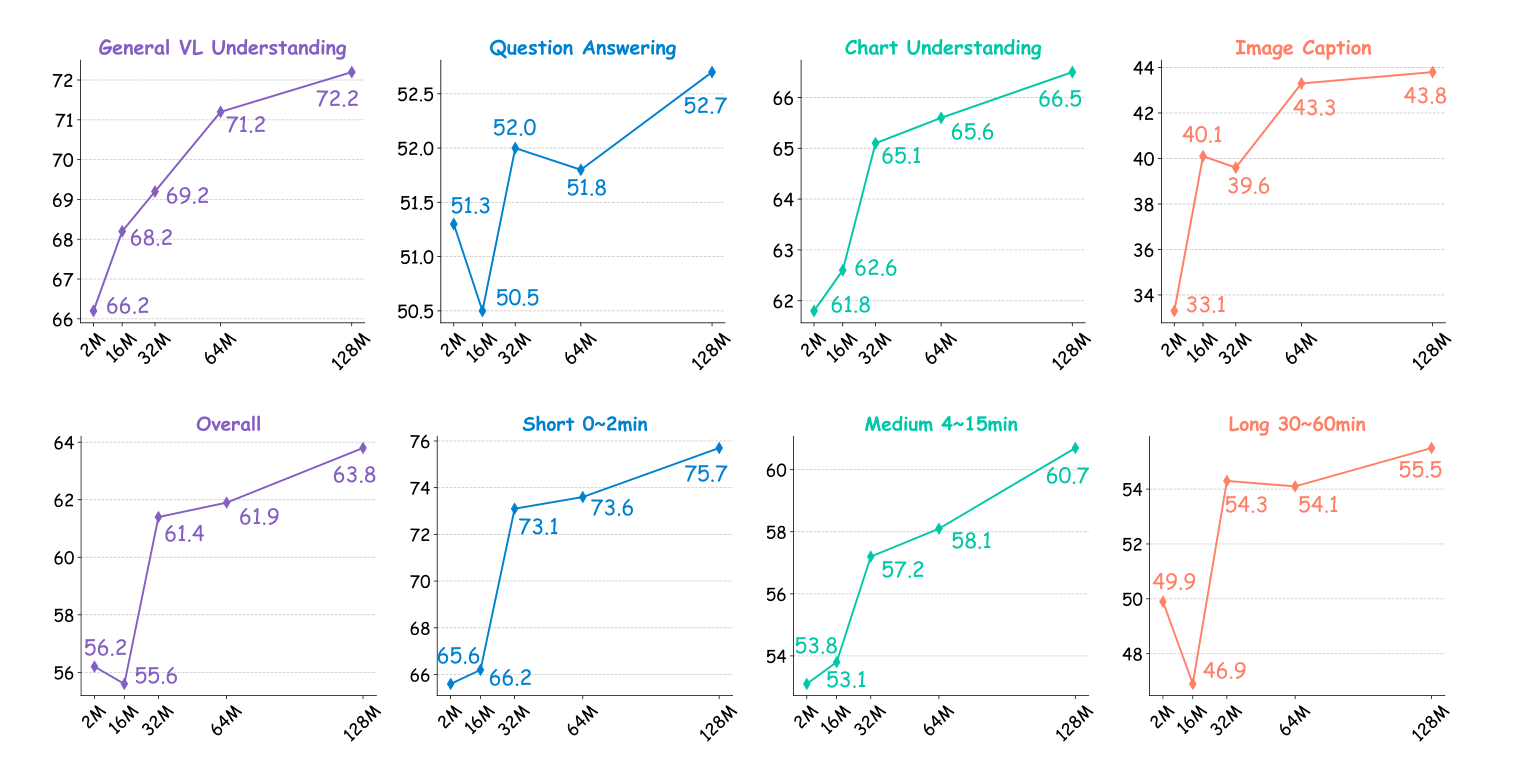
\includegraphics[width=0.86\textwidth]{figs/p4_scaling.png}
\caption{Effect of scaling video pretraining data \cite{p4}}
\label{fig:p4_scale}
\end{figure}

\paragraph{} \textbf{Comparison.} The video-pretrained 1B encoder averages 78.5\% zero-shot accuracy across 27 classification datasets, against 72.4\% for the EVA-01-CLIP-g/14 it starts from, outperforming the 6B InternVL-C encoder. LLaVA-Prime-7B surpasses LLaVA-OneVision-7B on both image and video benchmarks, and video pretraining of the LLM even improves pure-text scores, by 3.4 points on CMMLU \cite{p4}.

{\renewcommand{\arraystretch}{1.12}
\begin{table}[htbp]
\centering
\caption{LLaVA-Prime ablation and comparison}\label{tab:p4_res}
\small
\setlength{\tabcolsep}{4pt}
\begin{tabular}{|l|c|c|c|c|}
\hline
\textbf{Model} & \textbf{MME} & \textbf{MMBench} & \textbf{EgoSchema} & \textbf{Video-MME} \\ \hline
LLaVA-1.5 (ViT-g + Qwen2-7B) & 1569 & 70.6 & 45.0 & 55.1 \\ \hline
+ Stage I video pretraining & 1603 & 74.3 & 51.2 & 57.5 \\ \hline
+ Stage II video pretraining & 1621 & 73.5 & 52.4 & 58.8 \\ \hline
+ Stage III with CHA & 1610 & 73.6 & 54.3 & 60.2 \\ \hline
LLaVA-OneVision-7B & 1580 & 80.8 & 60.1 & 58.2 \\ \hline
LLaVA-Prime-7B & 1664 & 81.2 & 62.6 & 63.8 \\ \hline
\end{tabular}
\end{table}}

\subsection{Discussion}

\paragraph{} LLaVA-Prime shows that video is a scalable and data-efficient source of visual knowledge that benefits image tasks as well as video tasks, and that CHA makes video affordable by keeping token counts at image level. Its limitations are the very large compute budget, which few groups can reproduce; a modest margin over strong baselines on some image benchmarks; and some inconsistencies in reporting, such as 26 versus 27 datasets for the zero-shot average. Code and models are promised but were not yet available at publication.

% ---------------------------------------------------------------
\section{Summary of the Reviewed Papers}

\paragraph{} Table~\ref{tab:summary} summarises the four works; the next chapter compares them in detail.

{\renewcommand{\arraystretch}{1.15}
\begin{table}[htbp]
\centering
\caption{Summary of the reviewed works}\label{tab:summary}
\small
\begin{tabularx}{\textwidth}{|p{2.1cm}|p{2.4cm}|X|X|}
\hline
\textbf{Work} & \textbf{Problem} & \textbf{Technique} & \textbf{Main outcome} \\ \hline
Mirage \cite{p1} & Text-only reasoning on visual tasks & Latent visual tokens; two-stage SFT; GRPO & Better spatial reasoning and planning without generating images \\ \hline
AURORA \cite{p2} & Weak depth and counting perception & Depth and box perception tokens; distillation; curriculum & Large gains on harder depth and counting benchmarks \\ \hline
ZipVL \cite{p3} & Slow, memory-hungry LVLM inference & Adaptive important-token ratio; sparse attention; KV eviction & Faster prefill and decoding with near-full accuracy \\ \hline
LLaVA-Prime \cite{p4} & Costly, static image-text data & Four-stage video pretraining; causal hierarchical aggregation & Stronger image and video understanding \\ \hline
\end{tabularx}
\end{table}}

% ================= CHAPTER 4: DISCUSSION & COMPARISON =================
\chapter{Discussion \& Comparison}

\paragraph{} This chapter compares the four reviewed works. All build on the same vision-language architecture, but they target different weaknesses---reasoning, perception, efficiency, and training data---and intervene at different points of the pipeline. The comparison highlights their complementary strengths and the trade-offs among accuracy, cost, and generality.

\section{Analytical Focus and Methodology}

\paragraph{} Table~\ref{tab:cmp_method} compares the methodologies. Two works change \emph{what the model outputs while it reasons}: Mirage adds continuous latent visual tokens \cite{p1} and AURORA adds discrete perception tokens \cite{p2}. ZipVL changes \emph{how the model computes}, without any retraining \cite{p3}, and LLaVA-Prime changes \emph{what the model learns from}, through video pretraining \cite{p4}.

{\renewcommand{\arraystretch}{1.15}
\begin{table}[htbp]
\centering
\caption{Methodological comparison of the reviewed works}\label{tab:cmp_method}
\small
\begin{tabularx}{\textwidth}{|p{2.2cm}|X|X|X|X|}
\hline
\textbf{Aspect} & \textbf{Mirage \cite{p1}} & \textbf{AURORA \cite{p2}} & \textbf{ZipVL \cite{p3}} & \textbf{LLaVA-Prime \cite{p4}} \\ \hline
Target & Visual reasoning & Visual perception & Inference cost & Pretraining data \\ \hline
Base model & Qwen2.5-VL 7B, 3B & LLaVA 1.5 13B & LLaVA, LLaVA-Next, LongVA & ViT-g + Qwen2 7B, 72B \\ \hline
New element & Latent visual tokens & Depth and box tokens & Dynamic token sparsity & Video stages and CHA \\ \hline
Training & Two-stage SFT, GRPO & Distillation, curriculum & None & Four-stage pretraining \\ \hline
Inputs & Images & Images & Images, video & Images, video \\ \hline
Evaluation & VSP, Jigsaw, SAT, COMT & BLINK, CV-Bench, SEED & VQAv2, ChartQA, Video-MME & MME, MMBench, Video-MME \\ \hline
\end{tabularx}
\end{table}}

\section{Visual Tokens for Reasoning: Latent versus Explicit}

\paragraph{} Mirage and AURORA share the idea that a VLM should reason with visual intermediate steps, but they make opposite design choices. AURORA's perception tokens are \textbf{explicit and discrete}: they decode into depth maps or boxes, which makes them interpretable and lets them be supervised by specialist models, but each depth map costs 100 tokens and the vocabulary must be extended for every new kind of intrinsic \cite{p2}. Mirage's latent tokens are \textbf{implicit and continuous}: only four vectors, anchored to the visual subspace in Stage 1 and then freed to serve the answer in Stage 2, so they are cheaper and more flexible but cannot be inspected directly \cite{p1}. Mirage reports that AURORA-style explicit generation performs poorly on interleaved spatial planning, suggesting that compact latent cues suit multi-step reasoning, while explicit tokens remain attractive when the intermediate result itself---a depth map or a set of boxes---is useful.

\section{Efficiency and Scalability}

\paragraph{} The works sit at opposite ends of the cost spectrum. ZipVL \emph{reduces} inference cost with no training, keeping roughly 30--50\% of tokens and achieving up to 2.3 times faster prefill and 2.8 times higher decoding throughput \cite{p3}. LLaVA-Prime \emph{increases} training cost substantially---hundreds of GPUs for weeks---but CHA keeps inference cost at image level by compressing video tokens \cite{p4}. Mirage and AURORA add modest inference cost, four latent tokens or about a hundred perception tokens, in exchange for better reasoning. These approaches are complementary: a model pretrained with video, reasoning with latent or perception tokens, could be served with dynamic token sparsity.

\section{Training Data and Supervision}

\paragraph{} All four works depend on data engineering. Mirage synthesises helper images with tools and reasoning traces with a larger VLM \cite{p1}; AURORA generates pseudo-depth maps with Depth Anything and boxes from LVIS \cite{p2}; and LLaVA-Prime relies on 32M to 128M automatically captioned videos from Panda-70M \cite{p4}. Synthetic supervision is cheap and scalable but can be noisy---Mirage notes that video-generated helper images for SAT lack ground truth---and none of the works studies how errors in synthetic data affect reliability.

\section{Strengths and Limitations}

\paragraph{} Table~\ref{tab:cmp_sl} summarises the main strengths and limitations of each work. Every method improves one part of the VLM pipeline at a cost elsewhere: Mirage and AURORA add training effort and new tokens, ZipVL trades some accuracy on hard tasks for speed, and LLaVA-Prime trades a large training budget for broader visual knowledge.

{\renewcommand{\arraystretch}{1.15}
\begin{table}[htbp]
\centering
\caption{Strengths and limitations of the reviewed works}\label{tab:cmp_sl}
\small
\begin{tabularx}{\textwidth}{|p{2.2cm}|X|X|}
\hline
\textbf{Work} & \textbf{Strengths} & \textbf{Limitations} \\ \hline
Mirage \cite{p1} & No image decoder; only four latent tokens; transfers to smaller models; ablation-backed design & Relies on synthetic helper images and traces; small spatial benchmarks; latent tokens not interpretable \\ \hline
AURORA \cite{p2} & Interpretable depth and box tokens; no external tools at inference; extensible to new intrinsics & Two tasks on one base model; long token sequences; trails closed-source models on counting \\ \hline
ZipVL \cite{p3} & Training-free; works with FlashAttention; one signal drives prefill and decoding savings & Attention-only sparsity; probe overhead at short lengths; accuracy loss on hard tasks \\ \hline
LLaVA-Prime \cite{p4} & Scalable video data; benefits image and video tasks; token count kept at image level & Very large compute budget; modest gains on some benchmarks; reporting inconsistencies \\ \hline
\end{tabularx}
\end{table}}

\section{Evaluation and Overall Insights}

\paragraph{} The evaluations differ in scope. Mirage and AURORA use small, targeted benchmarks of spatial reasoning, depth, and counting, with roughly a thousand training examples per task; ZipVL and LLaVA-Prime evaluate on broad image and video suites. Gains are therefore not directly comparable. Taken together, the works show a consistent pattern. \textbf{First}, giving VLMs visual intermediate representations---latent or explicit---improves tasks that language alone handles poorly. \textbf{Second}, much of a VLM's visual input is redundant, so adaptive sparsity can cut cost with little loss. \textbf{Third}, richer data such as video improves even static image understanding. \textbf{Fourth}, these advances are complementary, so combining them in one system is the natural next step.

\section{Towards a Combined System}

\paragraph{} Because the four works act at different stages, they can in principle be combined, as sketched in Figure~\ref{fig:combined}. A vision encoder and LLM pretrained on video with causal hierarchical aggregation would supply temporal and static visual knowledge \cite{p4}; during inference, dynamic token sparsity would keep only the important visual tokens and shrink the KV cache \cite{p3}; and while generating its answer, the model would insert perception tokens when an explicit depth map or set of boxes is useful \cite{p2} and latent visual tokens when it needs to imagine a step \cite{p1}. Whether these gains add up, and how sparsity interacts with latent reasoning, has not yet been tested and is a natural direction for future work.

\begin{figure}[htbp]
\centering
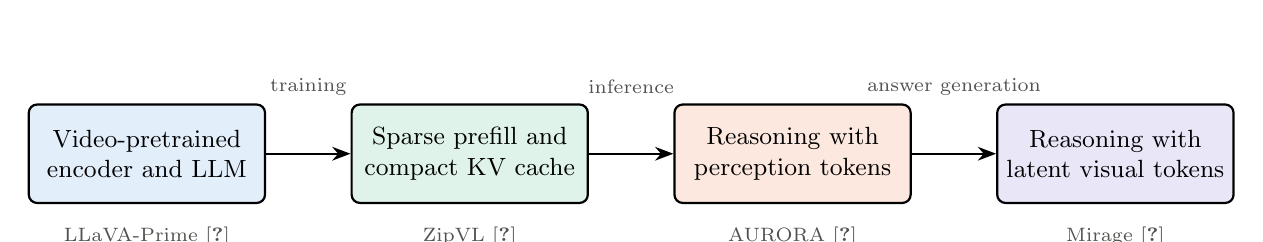
\begin{tikzpicture}[>=Stealth, thick,
  stage/.style={draw, rounded corners=3pt, minimum width=3.0cm, minimum height=1.25cm, font=\small, align=center},
  src/.style={font=\scriptsize, text=inkgray, align=center}]
\node[stage, fill=boxblue] (s1) at (0,0) {Video-pretrained\\ encoder and LLM};
\node[stage, fill=boxgreen] (s2) at (4.1,0) {Sparse prefill and\\ compact KV cache};
\node[stage, fill=boxorange] (s3) at (8.2,0) {Reasoning with\\ perception tokens};
\node[stage, fill=boxviolet] (s4) at (12.3,0) {Reasoning with\\ latent visual tokens};
\draw[->] (s1) -- (s2); \draw[->] (s2) -- (s3); \draw[->] (s3) -- (s4);
\node[src] at (0,-1.05) {LLaVA-Prime \cite{p4}};
\node[src] at (4.1,-1.05) {ZipVL \cite{p3}};
\node[src] at (8.2,-1.05) {AURORA \cite{p2}};
\node[src] at (12.3,-1.05) {Mirage \cite{p1}};
\node[font=\scriptsize, text=inkgray] at (2.05,0.85) {training};
\node[font=\scriptsize, text=inkgray] at (6.15,0.85) {inference};
\node[font=\scriptsize, text=inkgray] at (10.25,0.85) {answer generation};
\end{tikzpicture}
\caption{A combined pipeline using all four reviewed ideas}
\label{fig:combined}
\end{figure}

% ================= CHAPTER 5: APPLICATIONS =================
\chapter{Applications}

\section{Robotics and Embodied AI}

\paragraph{} Robots must plan paths, grasp objects, and judge distances. Latent visual reasoning improves spatial planning \cite{p1}, perception tokens add depth awareness \cite{p2}, and efficient inference makes on-board deployment feasible \cite{p3}.

\section{Autonomous Systems and Surveillance}

\paragraph{} Vehicles, drones, and cameras process long video streams in real time. Video-pretrained VLMs understand events and motion \cite{p4}, while dynamic token sparsity reduces latency and memory for long inputs \cite{p3}.

\section{Healthcare and Assistive Technology}

\paragraph{} VLMs can describe medical images, answer clinicians' questions, and help visually impaired people understand their surroundings. Reliable counting and spatial reasoning \cite{p1,p2} are important for such safety-critical uses.

\section{Document, Chart, and Education Tools}

\paragraph{} Chart and document understanding, which ZipVL evaluates with ChartQA and TextVQA \cite{p3}, supports report analysis and tutoring, and step-by-step visual reasoning \cite{p1} helps explain answers to students.

% ================= CHAPTER 6: CHALLENGES AND FUTURE DIRECTIONS =================
\chapter{Challenges and Future Directions}

\section{Challenges Identified in the Reviewed Works}

\paragraph{} \textbf{Mirage \cite{p1}} depends on synthesised helper images and traces and is tested on four spatial benchmarks. \textbf{AURORA \cite{p2}} covers only depth and counting on one base model and trails closed-source models on counting. \textbf{ZipVL \cite{p3}} sparsifies only attention and still loses accuracy on hard tasks such as ChartQA. \textbf{LLaVA-Prime \cite{p4}} requires a very large compute budget that few groups can reproduce.

\section{Cross-Cutting Challenges}

\paragraph{} The field faces \textbf{interpretability} limits, since latent tokens are hard to inspect; \textbf{hallucination}, where VLMs describe things that are not present; \textbf{data quality}, as synthetic supervision can be noisy; \textbf{evaluation gaps}, with small or inconsistent benchmarks; and \textbf{compute cost} for training and serving large models.

\section{Future Research Directions}

\paragraph{} Promising directions are \textbf{unified systems} that combine video pretraining, latent or perception-token reasoning, and sparse inference; \textbf{interpretable latent reasoning} that can decode latent tokens when needed; \textbf{extending sparsity} to MLP layers \cite{p3}; \textbf{broader perception tokens} for segmentation, pose, and motion \cite{p2}; and \textbf{efficient video learning} with fewer GPUs \cite{p4}.

% ================= CHAPTER 7: CONCLUSION =================
\chapter{Conclusion}

\paragraph{} Multimodal AI connects computer vision with language-based understanding, and vision-language models have become its central tool. This seminar reviewed four recent works that address their main limitations. \textbf{Mirage} \cite{p1}, the base paper, lets VLMs reason with compact latent visual tokens instead of generating images, improving spatial reasoning and planning. \textbf{AURORA} \cite{p2} adds depth and bounding-box perception tokens as intermediate reasoning steps, improving relative depth estimation and counting. \textbf{ZipVL} \cite{p3} selects important tokens dynamically in each layer, accelerating prefill and decoding with little loss of accuracy. \textbf{LLaVA-Prime} \cite{p4} pretrains VLMs on large-scale video with causal hierarchical aggregation, strengthening both image and video understanding.

\paragraph{} The comparison shows that visual intermediate representations improve reasoning that language alone handles poorly, that adaptive sparsity removes much of the redundancy in visual input, and that video is a rich, scalable source of training data. Because these advances act at different points of the same pipeline, they are complementary. The field is therefore moving towards multimodal systems that perceive richly, reason visually, and run efficiently---combining latent reasoning, perception-aware learning, efficient computation, and better data to build more accurate, efficient, and reliable multimodal intelligence.

% ================= REFERENCES =================
\begingroup
\setstretch{1.15}
\begin{thebibliography}{99}
\addcontentsline{toc}{chapter}{References}

\bibitem{p1}
Z. Yang, X. Yu, D. Chen, M. Shen, and C. Gan, ``Machine mental imagery: Empower multimodal reasoning with latent visual tokens,'' in \textit{Proc. IEEE/CVF Conf. Computer Vision and Pattern Recognition}, 2026, pp. 33510--33520.

\bibitem{p2}
M. Bigverdi, Z. Luo, C.-Y. Hsieh, E. Shen, \textit{et al.}, ``Perception tokens enhance visual reasoning in multimodal language models,'' in \textit{Proc. IEEE/CVF Conf. Computer Vision and Pattern Recognition}, 2025, pp. 3836--3845.

\bibitem{p3}
Y. He, F. Chen, J. Liu, W. Shao, \textit{et al.}, ``ZipVL: Accelerating vision-language models through dynamic token sparsity,'' in \textit{Proc. IEEE/CVF Int. Conf. Computer Vision}, 2025, pp. 20477--20486.

\bibitem{p4}
Y. Zhang, H. Li, J. Liu, and X. Yue, ``Learning beyond still frames: Scaling vision-language models with video,'' in \textit{Proc. IEEE/CVF Int. Conf. Computer Vision}, 2025, pp. 22425--22435.

\bibitem{radford2021}
A. Radford, J. W. Kim, C. Hallacy, A. Ramesh, G. Goh, S. Agarwal, \textit{et al.}, ``Learning transferable visual models from natural language supervision,'' in \textit{Proc. Int. Conf. Machine Learning}, 2021, pp. 8748--8763.

\bibitem{liu2023}
H. Liu, C. Li, Q. Wu, and Y. J. Lee, ``Visual instruction tuning,'' in \textit{Advances in Neural Information Processing Systems}, vol. 36, 2023.

\bibitem{dosovitskiy2021}
A. Dosovitskiy, L. Beyer, A. Kolesnikov, \textit{et al.}, ``An image is worth 16x16 words: Transformers for image recognition at scale,'' in \textit{Proc. Int. Conf. Learning Representations}, 2021.

\bibitem{vaswani2017}
A. Vaswani, N. Shazeer, N. Parmar, J. Uszkoreit, \textit{et al.}, ``Attention is all you need,'' in \textit{Advances in Neural Information Processing Systems}, vol. 30, 2017.

\bibitem{wei2022}
J. Wei, X. Wang, D. Schuurmans, M. Bosma, \textit{et al.}, ``Chain-of-thought prompting elicits reasoning in large language models,'' in \textit{Advances in Neural Information Processing Systems}, vol. 35, 2022, pp. 24824--24837.

\bibitem{oord2017}
A. van den Oord, O. Vinyals, and K. Kavukcuoglu, ``Neural discrete representation learning,'' in \textit{Advances in Neural Information Processing Systems}, vol. 30, 2017.

\bibitem{shao2024}
Z. Shao, P. Wang, Q. Zhu, R. Xu, \textit{et al.}, ``DeepSeekMath: Pushing the limits of mathematical reasoning in open language models,'' arXiv preprint arXiv:2402.03300, 2024.

\end{thebibliography}
\endgroup

\end{document}
